\ProvidesFile{RoverReport.tex}

\documentclass[a4paper]{article}

\makeatletter
\def\ps@myPS{%
    \def\@oddfoot{\null\hfill\thepage}
    \def\@evenfoot{\thepage}%
    \def\@evenhead{\null\hfil\slshape\leftmark}%
    \def\@oddhead{{\slshape\rightmark}}}%
\makeatother

\pagestyle{myPS}

\usepackage{epsfig}
\usepackage{afterpage}
\usepackage{floatpag}
\usepackage{color}
\DeclareGraphicsRule{.pdftex}{pdf}{.pdftex}{}

\usepackage{caption}
\usepackage{subcaption}

\usepackage{hyperref}

\usepackage{float}

\usepackage{times}
\usepackage{natbib}
\usepackage{graphicx}
\usepackage{url}

\usepackage{amsmath,amssymb}
\usepackage{cases}
\usepackage{a4wide}
\usepackage{tikz}

\begin{document}

\setcounter{page}{1}
\pagenumbering{arabic}

\begin{titlepage}
\begin{center}

{\huge \bfseries Contact Jacobian Computation}

\vspace{2cm} 

\textsc{Jan Michalczyk} \\

\texttt{jan.michalczyk@inria.fr} \\[2cm] 

{March 31, 2014}

\vspace{2cm} 


\includegraphics[width=0.29\textwidth]{INRIA}

\end{center}
\end{titlepage}


\section{Introduction}

This document contains specification and documentation of the tests performed 
on the Exomars rover model using Siconos software. Model has been created using HuMAnS software and implemented using its C code generator. 
The intention thereof is a common reference and unification of mechanical tests of the exomars rover across different platforms. As of now, seven tests have been performed:

\begin{enumerate}

  \item Rover stabilization on a horizontal plane after a free-fall phase.\\[1mm]
        In the first test setting the rover falls freely from the height of 2 meters onto a horizontal plane.
        No torques are applied in any of the joints. The only external forces acting on the rover are
        the gravity and the ground reaction forces. Initial position of the rover has been set to (x, y, z) = (5, 5, 2) [m].
        Friction coefficient has been set to 0.7. This case has been divided into two sub-cases: first one with the normal restituion coefficient set to zero and
        the second one with the normal restitution coefficient set to 0.2. Tangential restitution coefficients have been set to zero in both sub-cases. 
  
  \item Rover stabilization on a horizontal plane with linearly varying velocity of one steering axis.\\[1mm]
        In the second test setting rover is dropped onto a horizontal plane and stands idle on it during the first 50 seconds of the simulation.
        After 50 seconds from the beginning of the simulation a constant torque $\tau = 0.00002Nm$ is applied in one of the steering axes (steering axis FL)
        causing its rotational motion with linear velocity. Wheel makes two full rotations around its vertical steering axis (FL). 
        Other external forces acting on the rover are the gravity and ground reaction. Initial position of the center of mass of the robot
        has been set to (x, y, z) = (5, 5, 2) [m]. Friction coefficient has been set to 0.4. Restitution coefficients (tangential and normal) have been set to zero.
        
  \item Rover stabilization on a horizontal plane with acceleration and deceleration phases.\\[1mm]
        In the third test setting rover's parcour is divided into six time intervals with different values of torques applied to the wheels:

        \begin{itemize} 
          \item $0s < t_s < 20s$, $\tau = 0Nm$           
          \item $20s < t_s < 40s$, $\tau = 0.0007Nm$        
          \item $40s < t_s < 80s$, $\tau = 0Nm$         
          \item $80s < t_s < 105s$, $\tau = -0.0007Nm$
          \item $105s < t_s < 150s$, $\tau = 0Nm$         
          \item $150s < t_s < 200s$, $\tau = -0.0005Nm$ 
        \end{itemize}

        \noindent Other external forces acting on the rover are the gravity and ground reactions. Initial position of the center of mass of the robot
        has been set to (x, y, z) = (5, 8, 0.57) [m]. In the $5^{th}$ phase rover effectively stops its motion until negative torques are applied.
        Friction coefficient has been set to 0.7. Restitution coefficients (tangential and normal) have been set to zero. 

  \item Rover stabilization on an inclined plane with a phase of upwards motion.\\[1mm]
        In the fourth test setting rover is set to stand steadily on an inclined plane.   
        Inclination angle of the slope has been set to 10$^\circ$. Torques applied to the wheels counterbalance torques caused by
        the gravity. After initial period higher torques are applied to the wheels which cause the robot to drive upwards. Blocking torques are equal to  
        $\tau_{b} = -0.87072Nm$. During the second phase of motion linearly varying torques are applied to all wheels.\\[1mm] 
        \noindent Rover's parcour has been devided into two phases:

        \begin{itemize} 
          \item $0s < t_s < 30s$, $\tau_{b}$ $-$  $constant$ $blocking$ $torques$           
          \item $30s < t_s < 40s$, $\tau_{m}$ $-$ $linearly$ $increasing$ $torques$        
        \end{itemize}

        Friction coefficient has been set to 0.8. Restitution coefficients (tangential and normal) have been set to zero. 

  \item Rover stabilization on an inclined plane with acceleration and deceleration phases.\\[1mm]
        In the fifth test setting rover is dropped onto the inclined plane.
        Inclination angle of the slope has been set to 10$^\circ$. After the 10$^{th}$ second of motion a simple PD controller
        is set using position and velocity of the center of mass in order to stop the rover on the slope. Rover stops effectively at $t = 25s$.
        Friction coefficient has been set to 0.8. Restitution coefficients (tangential and normal) have been set to zero. 

  \item Spherical obstacle crossing on a horizontal plane.\\[1mm] 
        In the sixth test setting rover is dropped onto the horizontal plane from the height of $2$ $m$. After $10$ $s$ linearly varying torques are applied to all wheels. 
        A spherical obstacle has been set in front of the rover. The obstacle is in the form of a sphere which protudes outside the plane.
        Center of the sphere has been set so that the protrusion is equal to $20$ $cm$. Coefficients of friction and restitution (normal) are in this case respectively:
        0.3 and 0. 

  \item Vertical step obstacle crossing.\\[1mm]
        In the seveth test setting rover is dropped onto a horizontal plane.
        An obstacle in the form of a horizontal step of height $0.1m$ (roughly equal to the wheel radius) has been set in front of the rover.
        At certain point of time ($t$ $=$ $10s$) rover starts moving towards the step and crosses it mounting on the higher plane.
        Friction coefficient has been set to 0.6. Restitution coefficient (normal) has been set to 0.1. 

\end{enumerate}

\noindent Results of each of the above tests  will be detailed in the following sections.\\[1mm]
\noindent In mechanical simulations with nonsmooth approach one is mostly interested in the following quantities:

\begin{itemize}
  \item $x_{COM}$ - mass center coordinates
  \item $x_{wheels}$ - wheels angular displacement 
  \item $v_{COM}$ - mass center velocity
  \item $v_{wheels}$ - wheels angular velocity
  \item $R$ - reaction forces (impulsions) in lagrangian (global) coordinates
  \item $\lambda_{N}$ ($\lambda_{\bar{n}}$) - normal component of the contact force (impulsion) in local coordinates
  \item $\lambda_{T_x}$ ($\lambda_{\bar{t}}$) - tangential component of the contact force (impulsion) in local coordinates in the x direction
  \item $\lambda_{T_z}$ ($\lambda_{\bar{s}}$) - tangential component of the contact force (impulsion) in local coordinates in the z direction
  \item $y_{N}$ ($y_{\bar{n}}$) - gap function (distance between contact point and the constraint function)
  \item $\dot{y}_{N}$ ($\dot{y}_{\bar{n}}$) - normal component of the local contact velocity
  \item $\dot{y}_{T_x}$ ($\dot{y}_{\bar{t}}$) - tangential component x of the local contact velocity
  \item $\dot{y}_{T_z}$ ($\dot{y}_{\bar{s}}$) - tangential component z of the local contact velocity
\end{itemize}

\noindent For each scenario a subset of the above quantities has been plotted.\\

\begin{figure}[h!]
  \centering
    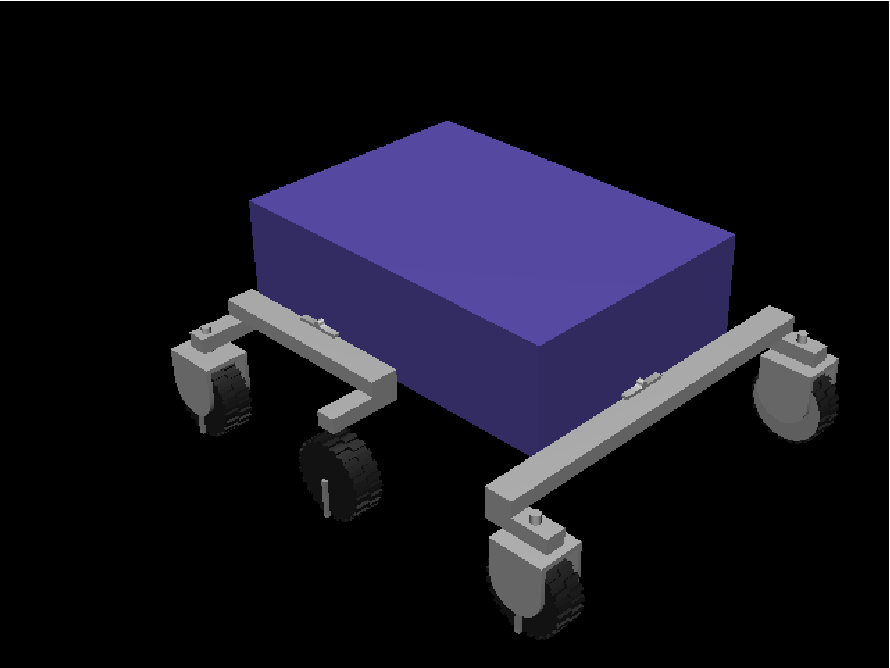
\includegraphics[width=0.8\textwidth]{rovereps}
  \caption{Assumed model of the robot}
\end{figure}

\newpage

\noindent Simplified kinematic structure of the robot is as follows:

\begin{figure}[h!]
  \centering
    \input{kkk.pdftex_t}  
  \caption{Geometry of the model}
\end{figure}

\newpage
\section{Test 1}
\label{Sec:test_1}

In the first test setting rover falls freely from the height of 1.5 meter onto the horizontal plane.
No torques are applied in any of the joints. The only external forces acting on the rover are
gravity and ground reaction forces. Initial position of the robot has been set to (x, y, z) = (10, 1.5, 10).

\begin{figure}[H]
  \centering
    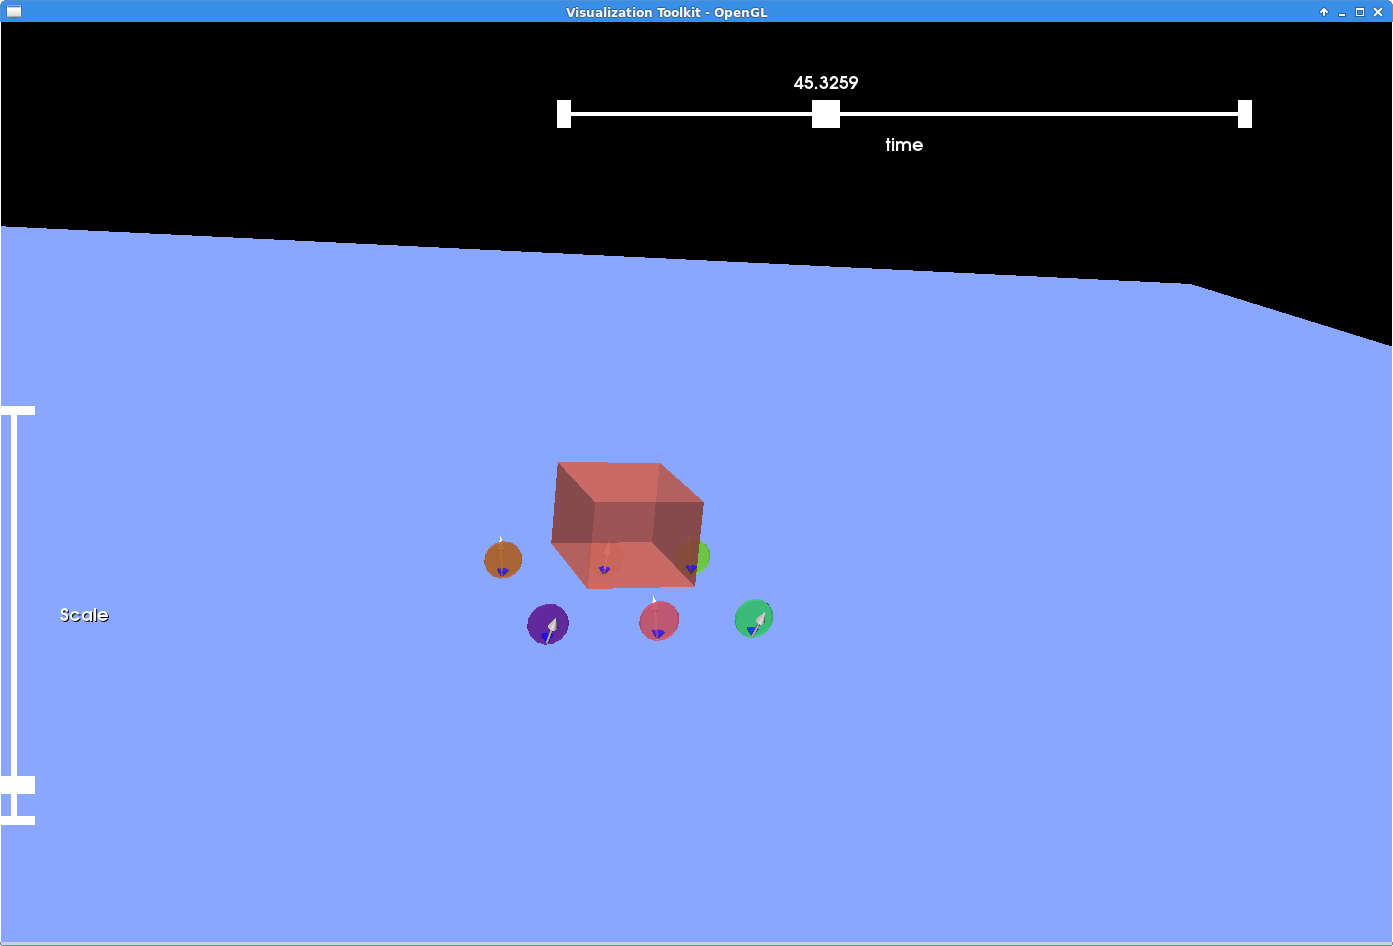
\includegraphics[width=0.8\textwidth]{run_1}
  \caption{First test setting}
\end{figure}

\noindent The following quantities have been plotted in this case:

\begin{itemize}
  \item $x_{COM}$ - mass centre coordinates
\end{itemize}

\begin{figure}[H]
  \centering
    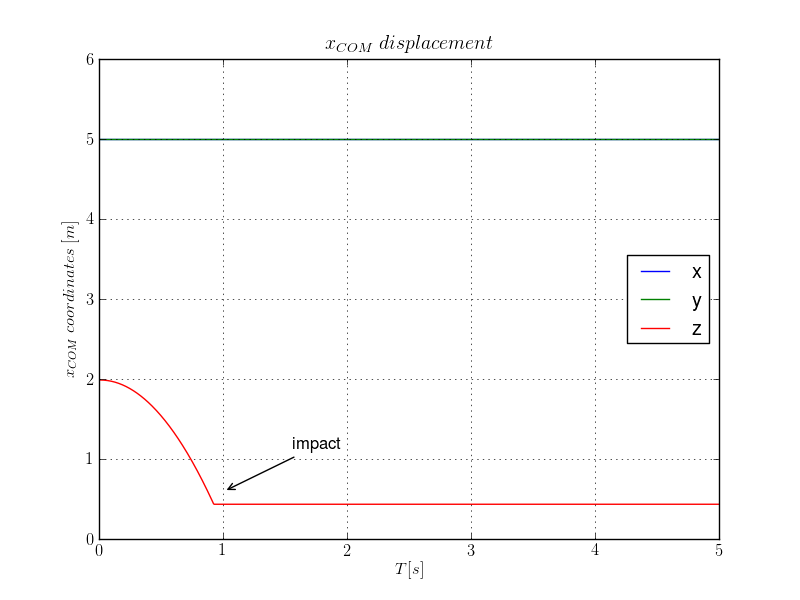
\includegraphics[width=0.8\textwidth]{xCOM}
  \caption{$x_{COM}$ displacement}
\end{figure}

\begin{itemize}
  \item $v_{COM}$ - mass centre velocity
\end{itemize}

\begin{figure}[H]
  \centering
    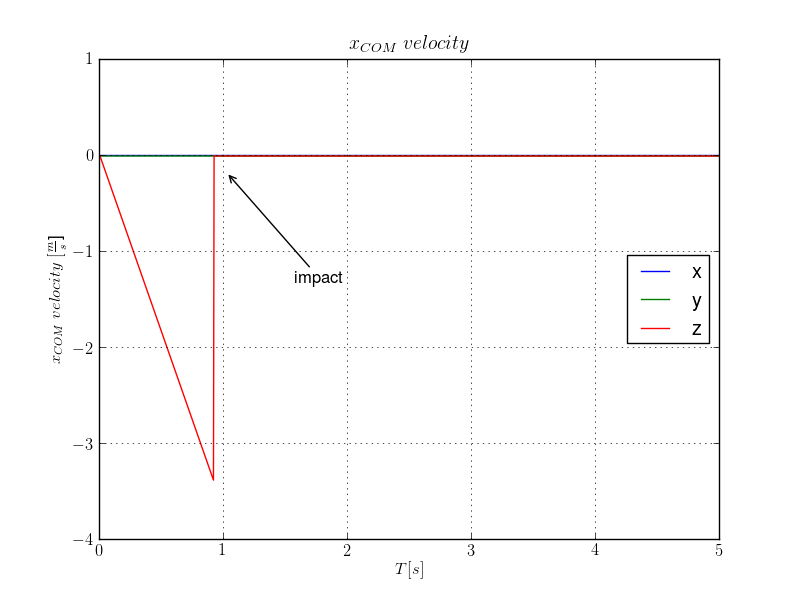
\includegraphics[width=0.8\textwidth]{vCOM}
  \caption{$x_{COM}$ velocity}
\end{figure}

\begin{itemize}
  \item $R$ - reaction forces in lagrangian coordinates for the center of mass
\end{itemize}

\begin{figure}[H]
  \centering
    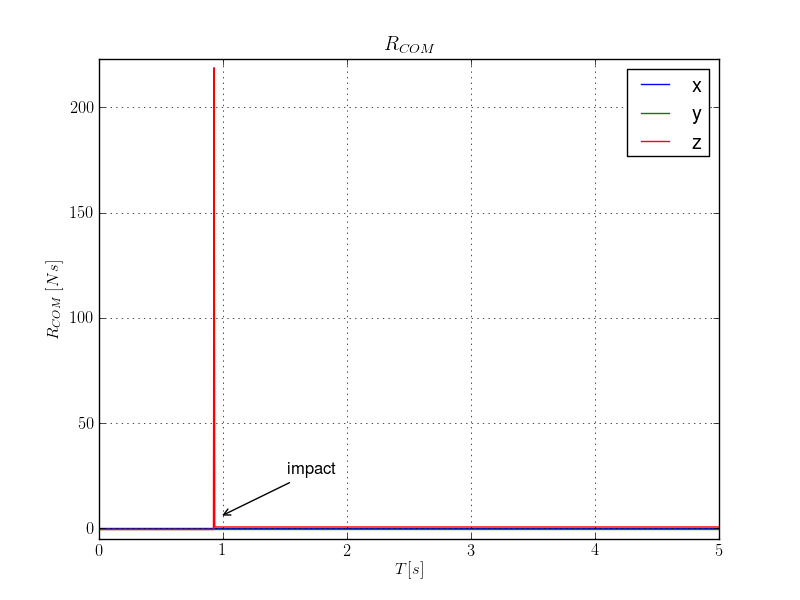
\includegraphics[width=0.8\textwidth]{p}
  \caption{$R$}
\end{figure}

\begin{itemize}
  \item $\lambda_{N}$ - normal component of the contact force (impulsion) for each wheel
\end{itemize}

\begin{figure}[H]
  \centering
    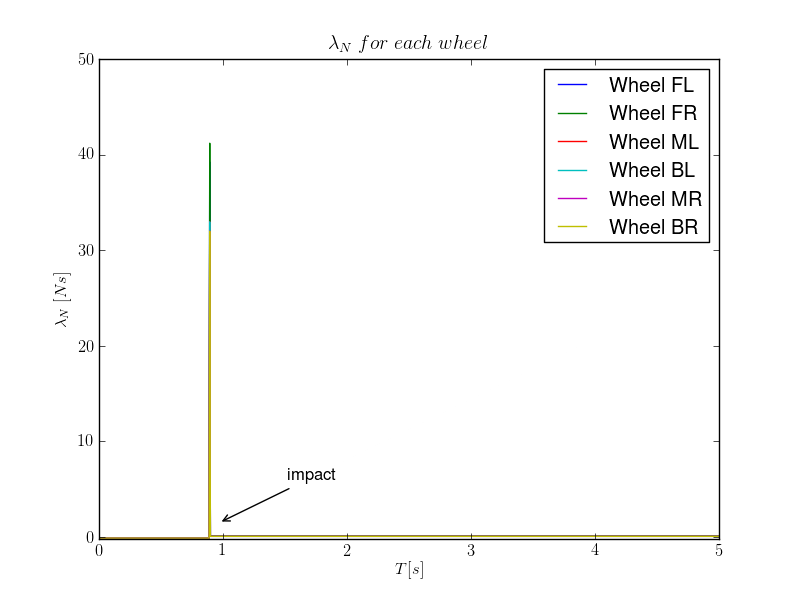
\includegraphics[width=0.8\textwidth]{lambdaN}
  \caption{$\lambda_{N}$ during impacts}
\end{figure}

\begin{figure}[H]
  \centering
    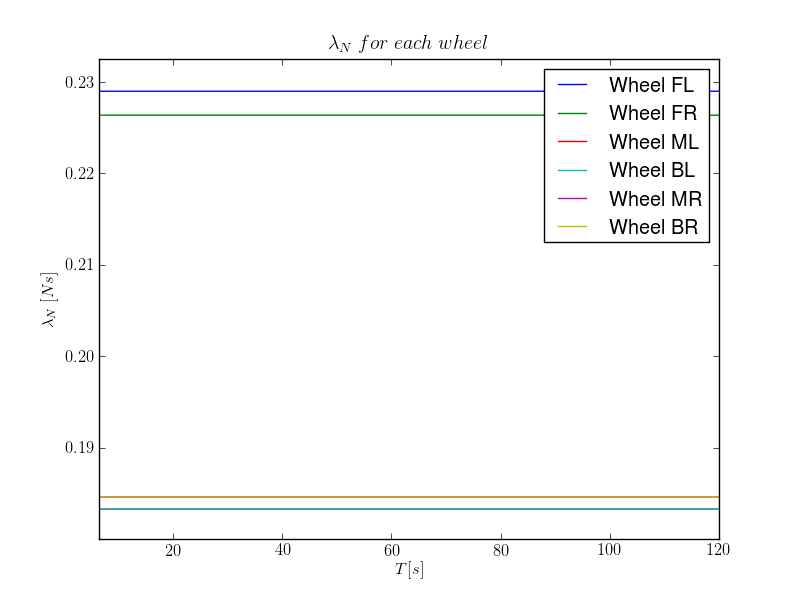
\includegraphics[width=0.8\textwidth]{lambdaNzoom}
  \caption{$\lambda_{N}$ zoom view of the steady state}
\end{figure}

\begin{itemize}
  \item $\lambda_{T_x}$ - tangential component of the contact force in the x direction for each wheel
\end{itemize}

\begin{figure}[H]
  \centering
    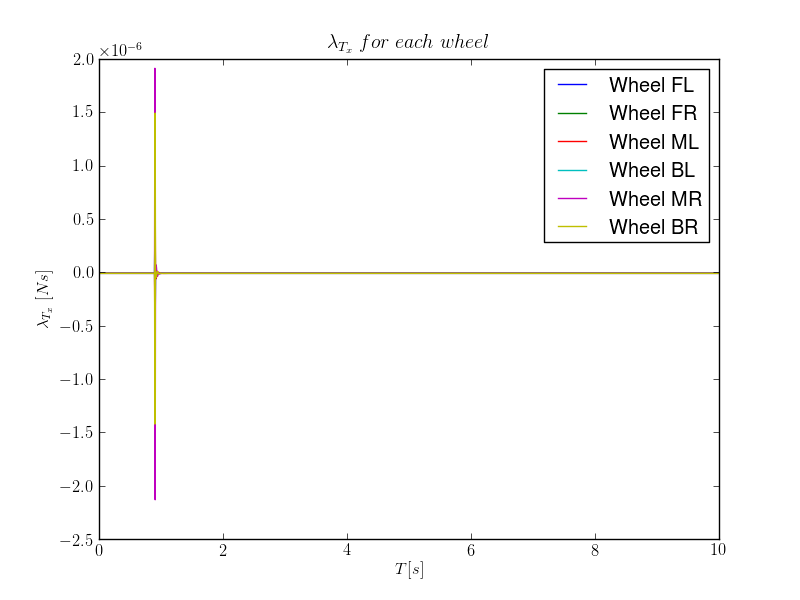
\includegraphics[width=0.8\textwidth]{lambdaTx}
  \caption{$\lambda_{T_x}$}
\end{figure}

\begin{itemize}
  \item $\lambda_{T_z}$ - tangential component of the contact force in the z direction for each wheel
\end{itemize}

\begin{figure}[H]
  \centering
    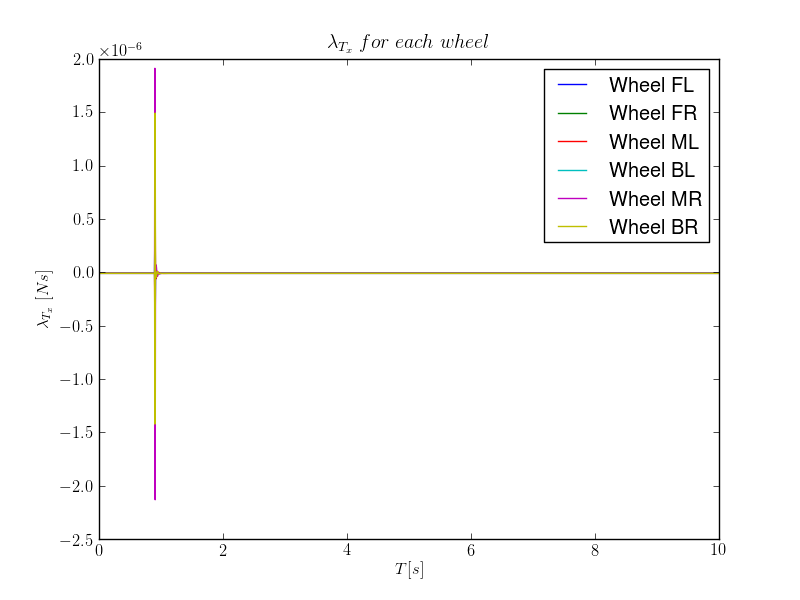
\includegraphics[width=0.8\textwidth]{lambdaTx}
  \caption{$\lambda_{T_z}$}
\end{figure}

\begin{itemize}
  \item $y_{N}$ - gap function (distance between contact point and the constraint function) for each wheel
\end{itemize}

\begin{figure}[H]
  \centering
    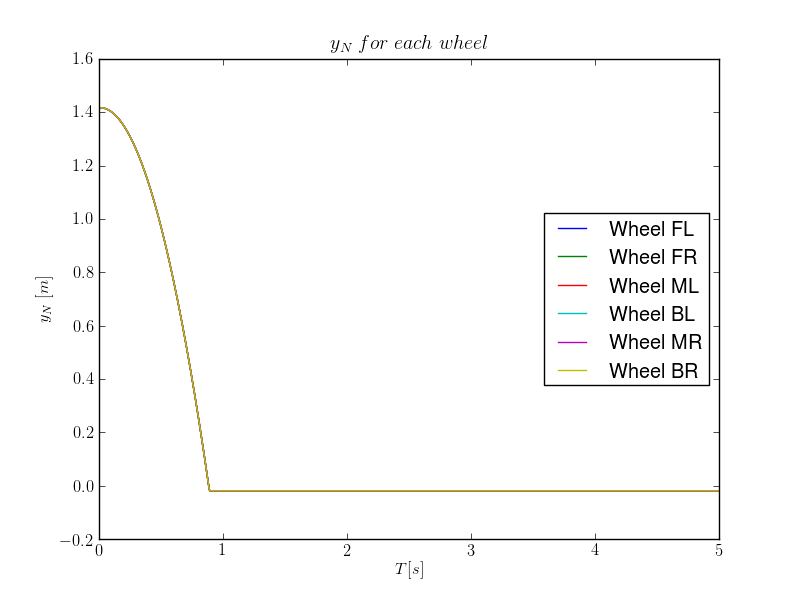
\includegraphics[width=0.8\textwidth]{yN}
  \caption{$y_{N}$}
\end{figure}

\begin{itemize}
  \item $\dot{y}_{N}$ - normal component of the local contact velocity for each wheel
\end{itemize}

\begin{figure}[H]
  \centering
    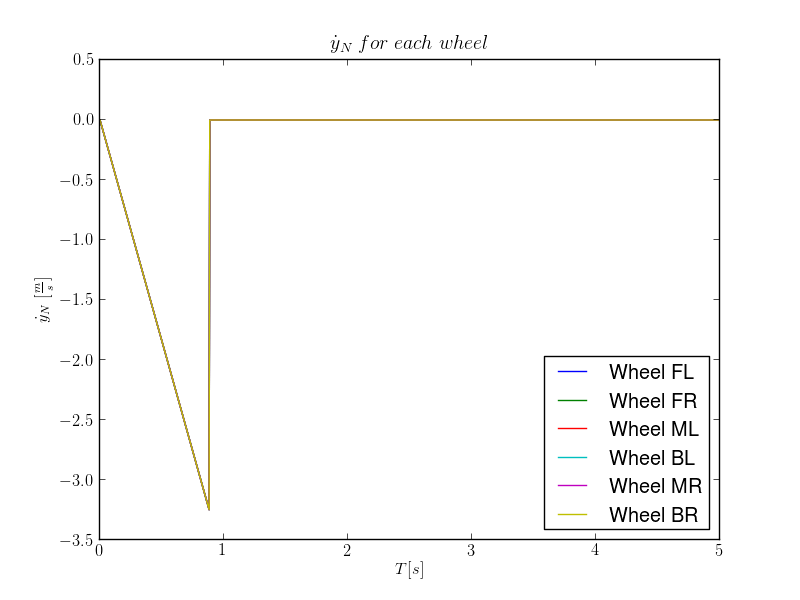
\includegraphics[width=0.8\textwidth]{yNdot}
  \caption{$\dot{y}_{N}$}
\end{figure}

\begin{itemize}
  \item $\dot{y}_{T_x}$ - tangential component x of the local contact velocity for each wheel
\end{itemize}

\begin{figure}[H]
  \centering
    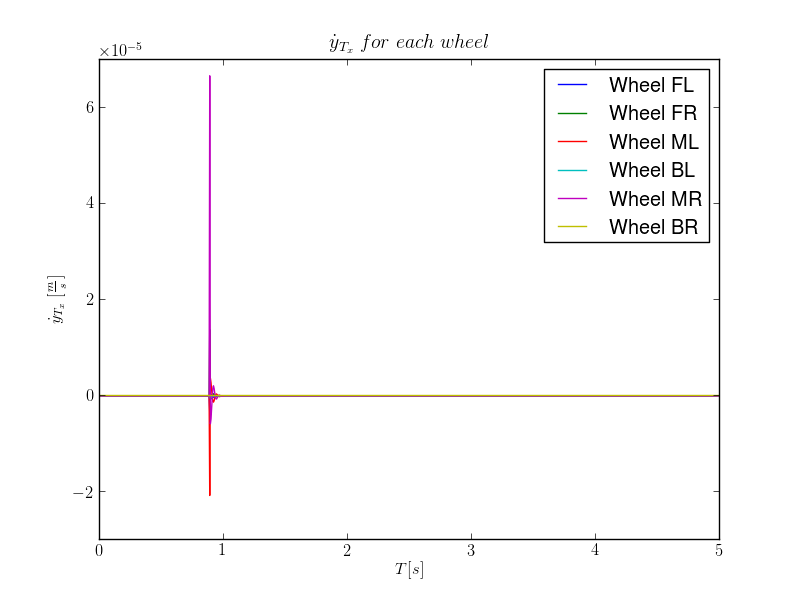
\includegraphics[width=0.8\textwidth]{yTxdot}
  \caption{$\dot{y}_{T_x}$}
\end{figure}

\begin{itemize}
  \item $\dot{y}_{T_z}$ - tangential component z of the local contact velocity for each wheel
\end{itemize}

\begin{figure}[H]
  \centering
    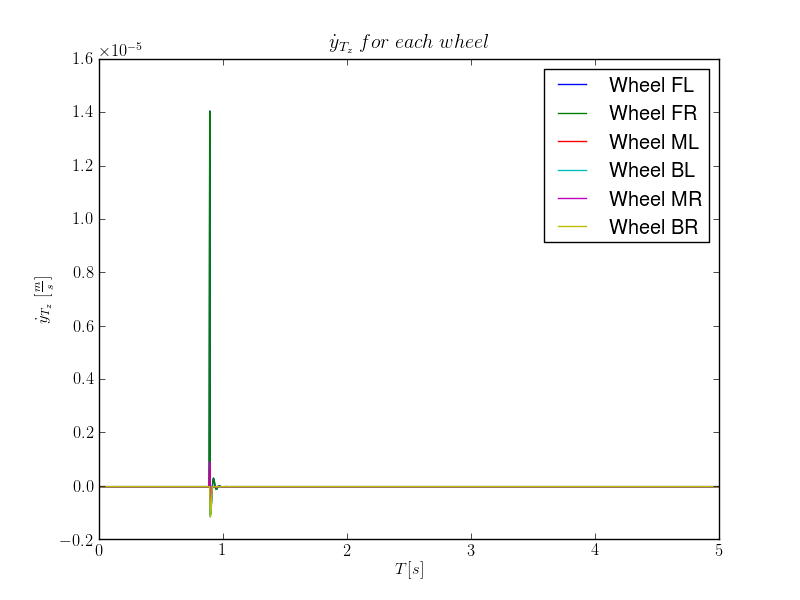
\includegraphics[width=0.8\textwidth]{yTzdot}
  \caption{$\dot{y}_{T_x}$}
\end{figure}

\noindent In the table below one can see last 100 values of $\lambda_{N}$ for each of the six wheels. Based on these values one can estimate the weight of the 
rover. 

\noindent By looking at the table one can see the values of $\lambda_{N}$ for front wheels are not equal for wheels FR and FL.\\

\noindent Based on the values from the table one can estimate the mass of the rover by summing up the six values of $\frac{\lambda_N}{timestep}$. Taking the 50$^{th}$ row of data
one finds that the weight of the robot is equal to $8632.80$ $kg$. If one divides it by the gravitational acceleration coefficient $g = 9.81$ $[\frac{m}{s^2}]$ one should obtain rover's mass estimate.

\noindent Estimate: $mass = 880.89$ $kg$. As given in the model definition: $mass = 960.00$ $kg$. 

\begin{center}
\resizebox{13.5cm}{!}{
\begin{tabular}{| c | c | c | c | c | c | c |}
\hline
t & $\lambda_N - FL$ & $\lambda_N - FR$ & $\lambda_N - ML$ & $\lambda_N - BL$ & $\lambda_N - MR$ & $\lambda_N - BR$ \\
\hline
249.5049999998456  & 7.871586034523761  & 8.53611984807527  & 6.855206982895642  & 6.855206982734339  & 6.522940076047917  & 6.522940075817996 \\
249.5099999998456  & 7.871586034523764  & 8.536119848075268  & 6.855206982895643  & 6.855206982734339  & 6.522940076047917  & 6.522940075817996 \\
249.5149999998456  & 7.871586034523762  & 8.536119848075272  & 6.855206982895643  & 6.855206982734339  & 6.522940076047917  & 6.522940075817996 \\
249.5199999998456  & 7.871586034523767  & 8.536119848075268  & 6.855206982895645  & 6.85520698273434  & 6.522940076047916  & 6.522940075817994 \\
249.5249999998456  & 7.871586034523762  & 8.53611984807527  & 6.855206982895643  & 6.855206982734339  & 6.522940076047914  & 6.522940075817994 \\
249.5299999998456  & 7.871586034523764  & 8.536119848075268  & 6.855206982895643  & 6.85520698273434  & 6.522940076047917  & 6.522940075817996 \\
249.5349999998456  & 7.871586034523762  & 8.53611984807527  & 6.855206982895645  & 6.85520698273434  & 6.522940076047917  & 6.522940075817996 \\
249.5399999998455  & 7.871586034523766  & 8.536119848075272  & 6.855206982895643  & 6.855206982734339  & 6.522940076047917  & 6.522940075817995 \\
249.5449999998455  & 7.871586034523767  & 8.536119848075268  & 6.855206982895643  & 6.855206982734339  & 6.522940076047916  & 6.522940075817995 \\
249.5499999998455  & 7.87158603452376  & 8.536119848075268  & 6.855206982895643  & 6.855206982734339  & 6.522940076047916  & 6.522940075817996 \\
249.5549999998455  & 7.871586034523763  & 8.536119848075268  & 6.855206982895643  & 6.855206982734339  & 6.522940076047917  & 6.522940075817995 \\
249.5599999998455  & 7.871586034523763  & 8.536119848075268  & 6.855206982895643  & 6.855206982734339  & 6.522940076047916  & 6.522940075817996 \\
249.5649999998455  & 7.871586034523764  & 8.53611984807527  & 6.855206982895643  & 6.855206982734339  & 6.522940076047917  & 6.522940075817996 \\
249.5699999998455  & 7.871586034523765  & 8.536119848075272  & 6.855206982895645  & 6.85520698273434  & 6.522940076047917  & 6.522940075817996 \\
249.5749999998455  & 7.871586034523768  & 8.53611984807527  & 6.855206982895643  & 6.85520698273434  & 6.522940076047917  & 6.522940075817995 \\
249.5799999998455  & 7.871586034523761  & 8.536119848075268  & 6.855206982895643  & 6.855206982734339  & 6.522940076047914  & 6.522940075817994 \\
249.5849999998455  & 7.871586034523765  & 8.536119848075268  & 6.855206982895643  & 6.855206982734339  & 6.522940076047916  & 6.522940075817995 \\
249.5899999998455  & 7.871586034523762  & 8.53611984807527  & 6.855206982895645  & 6.85520698273434  & 6.522940076047917  & 6.522940075817997 \\
249.5949999998455  & 7.871586034523767  & 8.536119848075272  & 6.855206982895643  & 6.855206982734339  & 6.522940076047917  & 6.522940075817996 \\
249.5999999998455  & 7.871586034523766  & 8.536119848075266  & 6.855206982895643  & 6.855206982734339  & 6.522940076047916  & 6.522940075817995 \\
249.6049999998455  & 7.87158603452376  & 8.53611984807527  & 6.855206982895643  & 6.855206982734339  & 6.522940076047916  & 6.522940075817996 \\
249.6099999998455  & 7.871586034523768  & 8.536119848075268  & 6.855206982895643  & 6.855206982734339  & 6.522940076047917  & 6.522940075817995 \\
249.6149999998455  & 7.871586034523762  & 8.53611984807527  & 6.855206982895643  & 6.855206982734339  & 6.522940076047916  & 6.522940075817996 \\
249.6199999998455  & 7.871586034523766  & 8.536119848075268  & 6.855206982895643  & 6.855206982734339  & 6.522940076047917  & 6.522940075817996 \\
249.6249999998455  & 7.871586034523763  & 8.53611984807527  & 6.855206982895645  & 6.85520698273434  & 6.522940076047917  & 6.522940075817996 \\
249.6299999998455  & 7.871586034523768  & 8.53611984807527  & 6.855206982895643  & 6.855206982734339  & 6.522940076047917  & 6.522940075817996 \\
249.6349999998455  & 7.871586034523764  & 8.53611984807527  & 6.855206982895643  & 6.855206982734339  & 6.522940076047917  & 6.522940075817996 \\
249.6399999998455  & 7.871586034523764  & 8.536119848075268  & 6.855206982895643  & 6.855206982734339  & 6.522940076047917  & 6.522940075817995 \\
249.6449999998455  & 7.871586034523763  & 8.536119848075268  & 6.855206982895643  & 6.855206982734339  & 6.522940076047916  & 6.522940075817996 \\
249.6499999998454  & 7.871586034523762  & 8.536119848075268  & 6.855206982895643  & 6.855206982734339  & 6.522940076047917  & 6.522940075817996 \\
249.6549999998454  & 7.871586034523766  & 8.53611984807527  & 6.855206982895644  & 6.855206982734341  & 6.522940076047917  & 6.522940075817995 \\
249.6599999998454  & 7.871586034523767  & 8.53611984807527  & 6.855206982895646  & 6.855206982734341  & 6.522940076047916  & 6.522940075817997 \\
249.6649999998454  & 7.871586034523766  & 8.536119848075272  & 6.855206982895643  & 6.855206982734338  & 6.522940076047917  & 6.522940075817994 \\
249.6699999998454  & 7.871586034523767  & 8.536119848075268  & 6.85520698289564  & 6.855206982734336  & 6.522940076047914  & 6.522940075817994 \\
249.6749999998454  & 7.87158603452376  & 8.536119848075266  & 6.85520698289564  & 6.855206982734338  & 6.522940076047916  & 6.522940075817996 \\
249.6799999998454  & 7.871586034523763  & 8.536119848075266  & 6.855206982895644  & 6.855206982734339  & 6.522940076047917  & 6.522940075817997 \\
249.6849999998454  & 7.871586034523764  & 8.536119848075268  & 6.855206982895643  & 6.855206982734338  & 6.522940076047917  & 6.522940075817995 \\
249.6899999998454  & 7.871586034523767  & 8.536119848075272  & 6.855206982895643  & 6.855206982734339  & 6.522940076047916  & 6.522940075817997 \\
249.6949999998454  & 7.871586034523767  & 8.536119848075268  & 6.855206982895643  & 6.855206982734339  & 6.522940076047917  & 6.522940075817997 \\
249.6999999998454  & 7.871586034523762  & 8.536119848075266  & 6.855206982895643  & 6.855206982734338  & 6.522940076047917  & 6.522940075817995 \\
249.7049999998454  & 7.871586034523764  & 8.536119848075268  & 6.855206982895641  & 6.855206982734338  & 6.522940076047914  & 6.522940075817994 \\
249.7099999998454  & 7.871586034523765  & 8.536119848075266  & 6.855206982895644  & 6.85520698273434  & 6.522940076047917  & 6.522940075817995 \\
249.7149999998454  & 7.871586034523764  & 8.53611984807527  & 6.855206982895644  & 6.855206982734339  & 6.522940076047916  & 6.522940075817996 \\
249.7199999998454  & 7.871586034523767  & 8.536119848075268  & 6.855206982895643  & 6.855206982734339  & 6.522940076047917  & 6.522940075817996 \\
249.7249999998454  & 7.871586034523764  & 8.53611984807527  & 6.855206982895643  & 6.855206982734339  & 6.522940076047917  & 6.522940075817996 \\
249.7299999998454  & 7.871586034523766  & 8.536119848075266  & 6.855206982895642  & 6.855206982734338  & 6.522940076047917  & 6.522940075817996 \\
249.7349999998454  & 7.871586034523763  & 8.536119848075268  & 6.855206982895642  & 6.855206982734338  & 6.522940076047917  & 6.522940075817996 \\
249.7399999998454  & 7.871586034523767  & 8.53611984807527  & 6.855206982895642  & 6.855206982734338  & 6.522940076047917  & 6.522940075817997 \\
249.7449999998454  & 7.871586034523767  & 8.536119848075266  & 6.855206982895642  & 6.855206982734338  & 6.522940076047918  & 6.522940075817996 \\
249.7499999998454  & 7.871586034523761  & 8.536119848075266  & 6.855206982895642  & 6.855206982734338  & 6.522940076047914  & 6.522940075817994 \\
249.7549999998454  & 7.871586034523766  & 8.536119848075268  & 6.855206982895644  & 6.85520698273434  & 6.522940076047916  & 6.522940075817996 \\
249.7599999998453  & 7.871586034523767  & 8.536119848075268  & 6.855206982895644  & 6.855206982734338  & 6.522940076047917  & 6.522940075817997 \\
249.7649999998453  & 7.871586034523764  & 8.536119848075268  & 6.855206982895641  & 6.855206982734337  & 6.522940076047917  & 6.522940075817996 \\
249.7699999998453  & 7.871586034523767  & 8.536119848075268  & 6.855206982895641  & 6.855206982734338  & 6.522940076047917  & 6.522940075817997 \\
249.7749999998453  & 7.871586034523764  & 8.536119848075266  & 6.855206982895642  & 6.855206982734337  & 6.522940076047917  & 6.522940075817996 \\
249.7799999998453  & 7.871586034523764  & 8.536119848075268  & 6.855206982895641  & 6.855206982734338  & 6.522940076047917  & 6.522940075817996 \\
249.7849999998453  & 7.871586034523767  & 8.536119848075266  & 6.855206982895644  & 6.85520698273434  & 6.522940076047917  & 6.522940075817996 \\
249.7899999998453  & 7.871586034523766  & 8.536119848075268  & 6.855206982895644  & 6.855206982734339  & 6.522940076047917  & 6.522940075817996 \\
249.7949999998453  & 7.871586034523766  & 8.53611984807527  & 6.855206982895642  & 6.855206982734337  & 6.522940076047917  & 6.522940075817996 \\
249.7999999998453  & 7.871586034523768  & 8.536119848075268  & 6.855206982895641  & 6.855206982734337  & 6.522940076047917  & 6.522940075817996 \\
249.8049999998453  & 7.871586034523766  & 8.536119848075268  & 6.855206982895641  & 6.855206982734338  & 6.522940076047917  & 6.522940075817997 \\
249.8099999998453  & 7.871586034523765  & 8.536119848075268  & 6.855206982895644  & 6.85520698273434  & 6.522940076047918  & 6.522940075817996 \\
249.8149999998453  & 7.871586034523768  & 8.536119848075268  & 6.855206982895643  & 6.855206982734339  & 6.522940076047916  & 6.522940075817996 \\
249.8199999998453  & 7.871586034523764  & 8.536119848075268  & 6.855206982895644  & 6.855206982734339  & 6.522940076047917  & 6.522940075817996 \\
249.8249999998453  & 7.871586034523767  & 8.53611984807527  & 6.855206982895642  & 6.855206982734338  & 6.522940076047917  & 6.522940075817997 \\
249.8299999998453  & 7.871586034523767  & 8.536119848075266  & 6.855206982895642  & 6.855206982734337  & 6.522940076047917  & 6.522940075817996 \\
249.8349999998453  & 7.871586034523764  & 8.536119848075266  & 6.855206982895641  & 6.855206982734339  & 6.522940076047917  & 6.522940075817997 \\
249.8399999998453  & 7.871586034523764  & 8.536119848075266  & 6.855206982895643  & 6.855206982734337  & 6.522940076047918  & 6.522940075817997 \\
249.8449999998453  & 7.871586034523765  & 8.536119848075266  & 6.855206982895641  & 6.855206982734337  & 6.522940076047916  & 6.522940075817996 \\
249.8499999998453  & 7.871586034523765  & 8.536119848075266  & 6.85520698289564  & 6.855206982734336  & 6.522940076047916  & 6.522940075817994 \\
249.8549999998453  & 7.871586034523765  & 8.536119848075264  & 6.855206982895641  & 6.855206982734337  & 6.522940076047916  & 6.522940075817996 \\
249.8599999998453  & 7.871586034523763  & 8.536119848075266  & 6.855206982895642  & 6.855206982734339  & 6.522940076047917  & 6.522940075817997 \\
249.8649999998453  & 7.871586034523768  & 8.536119848075268  & 6.855206982895645  & 6.855206982734339  & 6.522940076047917  & 6.522940075817997 \\
249.8699999998452  & 7.871586034523768  & 8.53611984807527  & 6.855206982895642  & 6.855206982734337  & 6.522940076047918  & 6.522940075817997 \\
249.8749999998452  & 7.871586034523768  & 8.536119848075268  & 6.855206982895639  & 6.855206982734336  & 6.522940076047916  & 6.522940075817994 \\
249.8799999998452  & 7.871586034523765  & 8.536119848075264  & 6.85520698289564  & 6.855206982734336  & 6.522940076047914  & 6.522940075817996 \\
249.8849999998452  & 7.871586034523763  & 8.536119848075263  & 6.855206982895642  & 6.855206982734338  & 6.522940076047918  & 6.522940075817996 \\
249.8899999998452  & 7.871586034523763  & 8.536119848075266  & 6.855206982895642  & 6.855206982734338  & 6.522940076047917  & 6.522940075817997 \\
249.8949999998452  & 7.871586034523768  & 8.536119848075268  & 6.855206982895643  & 6.855206982734338  & 6.522940076047918  & 6.522940075817997 \\
249.8999999998452  & 7.871586034523766  & 8.536119848075266  & 6.855206982895642  & 6.855206982734338  & 6.522940076047916  & 6.522940075817996 \\
249.9049999998452  & 7.871586034523765  & 8.536119848075268  & 6.855206982895642  & 6.855206982734338  & 6.522940076047917  & 6.522940075817996 \\
249.9099999998452  & 7.871586034523768  & 8.536119848075268  & 6.855206982895642  & 6.855206982734338  & 6.522940076047917  & 6.522940075817997 \\
249.9149999998452  & 7.871586034523766  & 8.536119848075266  & 6.855206982895642  & 6.855206982734336  & 6.522940076047917  & 6.522940075817996 \\
249.9199999998452  & 7.871586034523765  & 8.536119848075266  & 6.855206982895639  & 6.855206982734336  & 6.522940076047917  & 6.522940075817996 \\
249.9249999998452  & 7.871586034523765  & 8.536119848075266  & 6.855206982895642  & 6.855206982734339  & 6.522940076047917  & 6.522940075817996 \\
249.9299999998452  & 7.871586034523767  & 8.536119848075268  & 6.855206982895644  & 6.855206982734339  & 6.522940076047917  & 6.522940075817997 \\
249.9349999998452  & 7.871586034523767  & 8.536119848075268  & 6.855206982895643  & 6.855206982734339  & 6.522940076047917  & 6.522940075817996 \\
249.9399999998452  & 7.871586034523767  & 8.536119848075266  & 6.855206982895642  & 6.855206982734338  & 6.522940076047917  & 6.522940075817994 \\
249.9449999998452  & 7.871586034523765  & 8.536119848075266  & 6.855206982895642  & 6.855206982734338  & 6.522940076047914  & 6.522940075817996 \\
249.9499999998452  & 7.871586034523766  & 8.536119848075268  & 6.855206982895643  & 6.855206982734338  & 6.522940076047919  & 6.522940075817997 \\
249.9549999998452  & 7.871586034523766  & 8.536119848075266  & 6.85520698289564  & 6.855206982734336  & 6.522940076047917  & 6.522940075817996 \\
249.9599999998452  & 7.871586034523765  & 8.536119848075266  & 6.85520698289564  & 6.855206982734336  & 6.522940076047917  & 6.522940075817997 \\
249.9649999998452  & 7.871586034523766  & 8.536119848075266  & 6.855206982895641  & 6.855206982734337  & 6.522940076047917  & 6.522940075817996 \\
249.9699999998452  & 7.871586034523767  & 8.536119848075266  & 6.855206982895641  & 6.855206982734338  & 6.522940076047917  & 6.522940075817996 \\
249.9749999998452  & 7.871586034523766  & 8.536119848075268  & 6.855206982895644  & 6.855206982734339  & 6.522940076047917  & 6.522940075817996 \\
249.9799999998451  & 7.871586034523768  & 8.53611984807527  & 6.855206982895644  & 6.855206982734339  & 6.522940076047917  & 6.522940075817997 \\
249.9849999998451  & 7.871586034523768  & 8.536119848075268  & 6.855206982895642  & 6.855206982734338  & 6.522940076047917  & 6.522940075817996 \\
249.9899999998451  & 7.871586034523766  & 8.536119848075268  & 6.855206982895642  & 6.855206982734338  & 6.522940076047917  & 6.522940075817996 \\
249.9949999998451  & 7.871586034523766  & 8.536119848075266  & 6.855206982895642  & 6.855206982734336  & 6.522940076047917  & 6.522940075817996 \\
249.9999999998451  & 7.871586034523764  & 8.536119848075266  & 6.855206982895639  & 6.855206982734337  & 6.522940076047917  & 6.522940075817996 \\
\hline
\end{tabular}
}
\end{center}


\newpage
\section{Test 2}
\label{Sec:test_2}

In the second test setting rover is dropped onto a horizontal plane and stands idle on it during the first 50 seconds of the simulation.
After 50 seconds from the beginning of the simulation a constant torque $\tau = 0.00002Nm$ is applied in one of the steering axes (steering axis FL)
causing its rotational motion with linear velocity. Wheel makes two full rotations around its vertical steering axis (FL). 
Other external forces acting on the rover are the gravity and ground reaction. Initial position of the center of mass of the robot
has been set to (x, y, z) = (5, 5, 2) [m]. Friction coefficient has been set to 0.4. Restitution coefficients (tangential and normal) have been set to zero.

\begin{figure}[H]
  \centering
    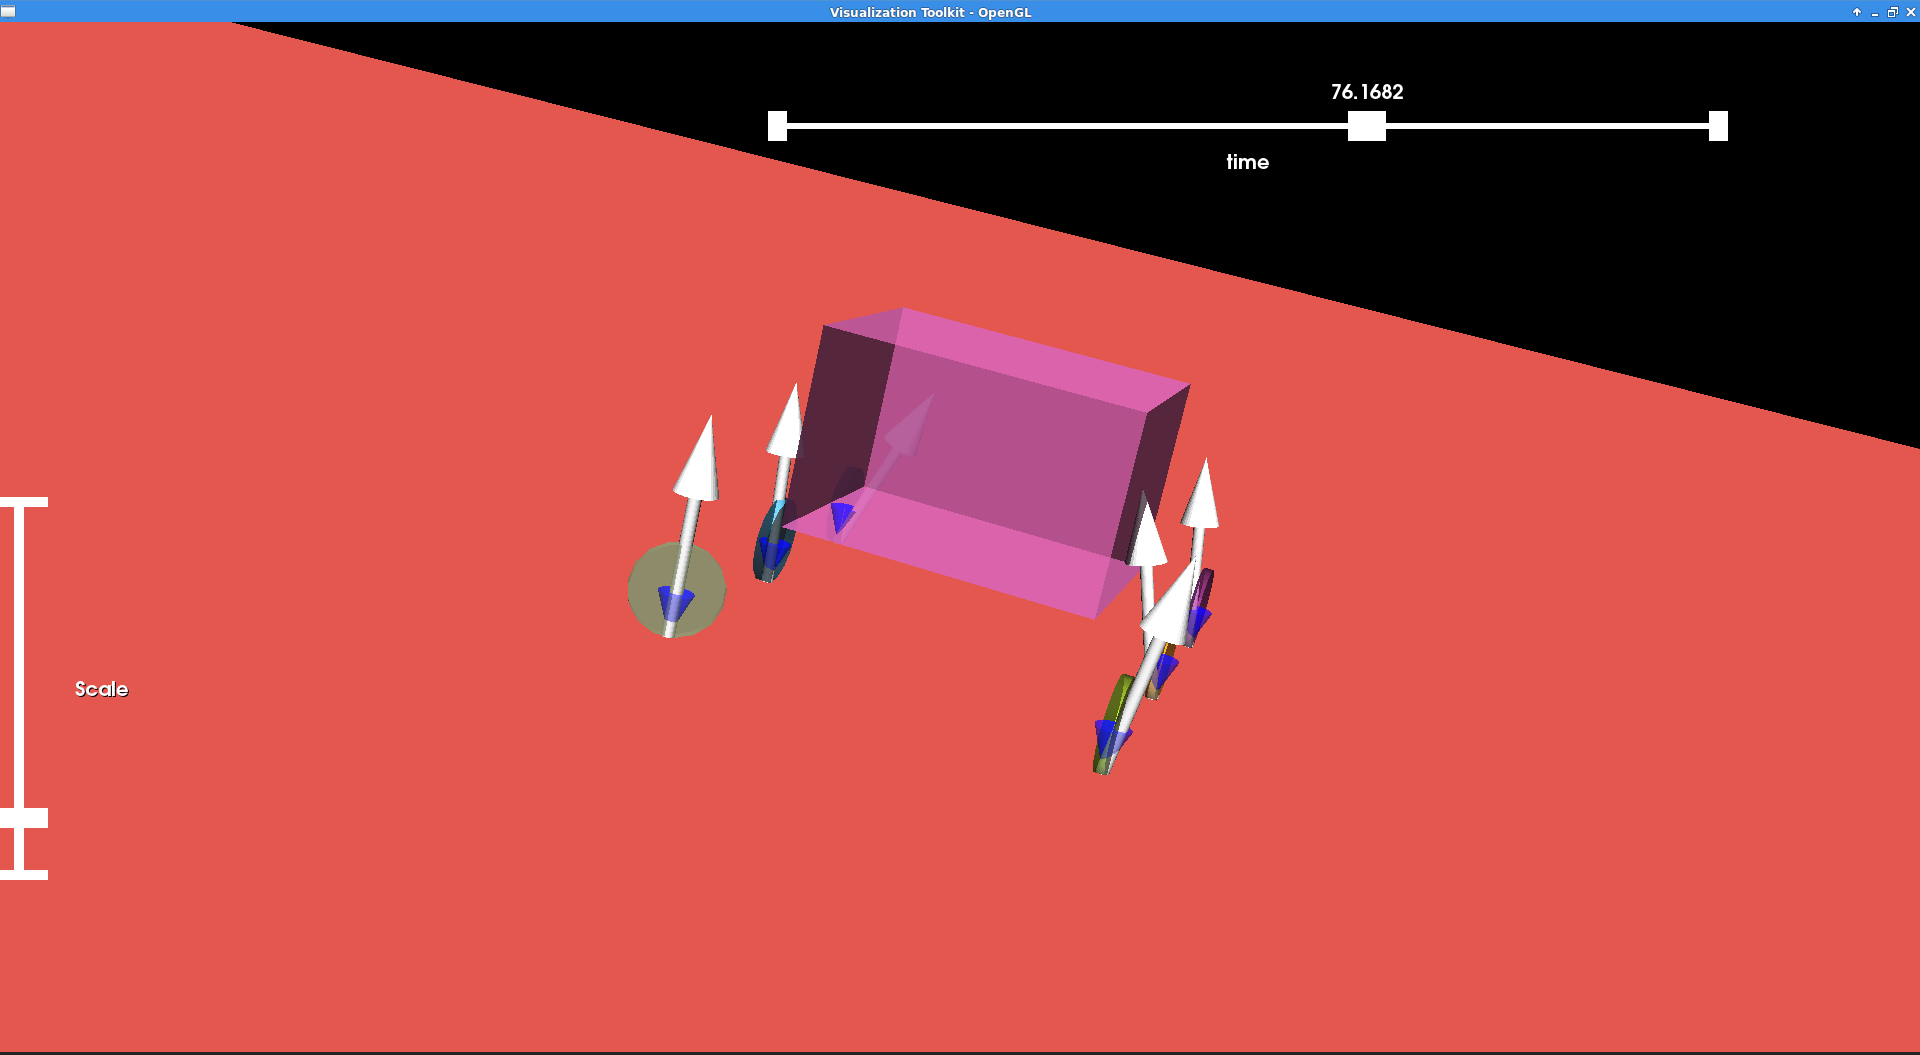
\includegraphics[width=0.8\textwidth]{run_2}
  \caption{Second test scenario (arrows depict contact forces)}
\end{figure}

\noindent In this case, following essential quantities have been plotted:

\begin{figure}[H]
  \centering
    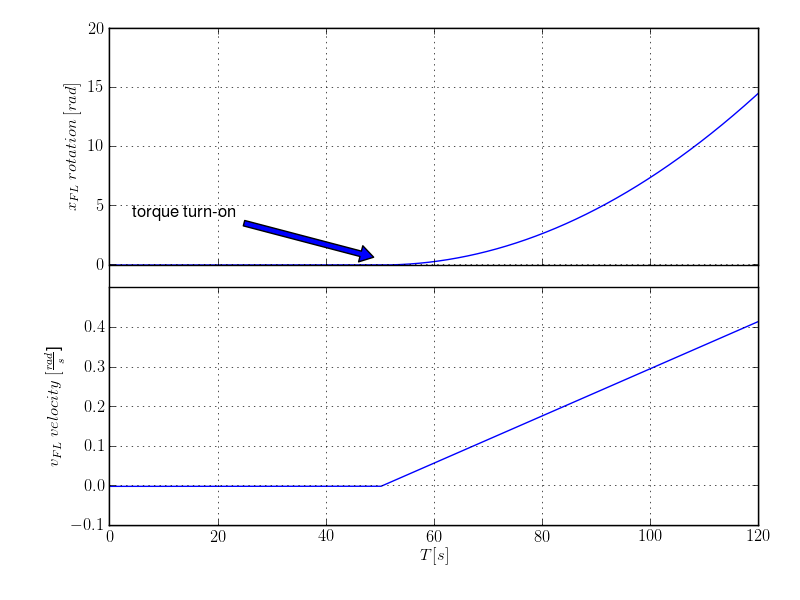
\includegraphics[width=0.8\textwidth]{xFLvFL}
  \caption{$x_{FL}$, $v_{FL}$ - angular displacement and velocity of the FL axis}
\end{figure}

\noindent \textbf{\textit{\Large{Comments}}}\\[1mm]
\noindent In the figure 11 one can see the variation of the steering axis displacement and velocity. After a constant torque is applied the axis is roatating with a linear velocity which corresponds to the quadratic
shape of the displacement cureve.\\

\noindent Also, the following complimentary quantities have been plotted:

\begin{figure}[H]
  \centering
    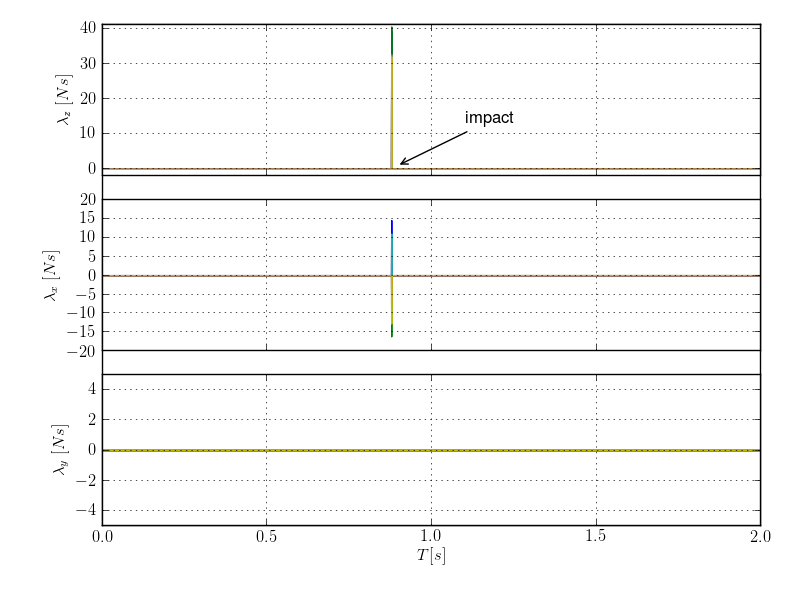
\includegraphics[width=0.8\textwidth]{lambdaNTS2}
  \caption{$\lambda_{N}$ - normal component of the contact force (impulsion) for each wheel}
\end{figure}

\begin{figure}[H]
  \centering
    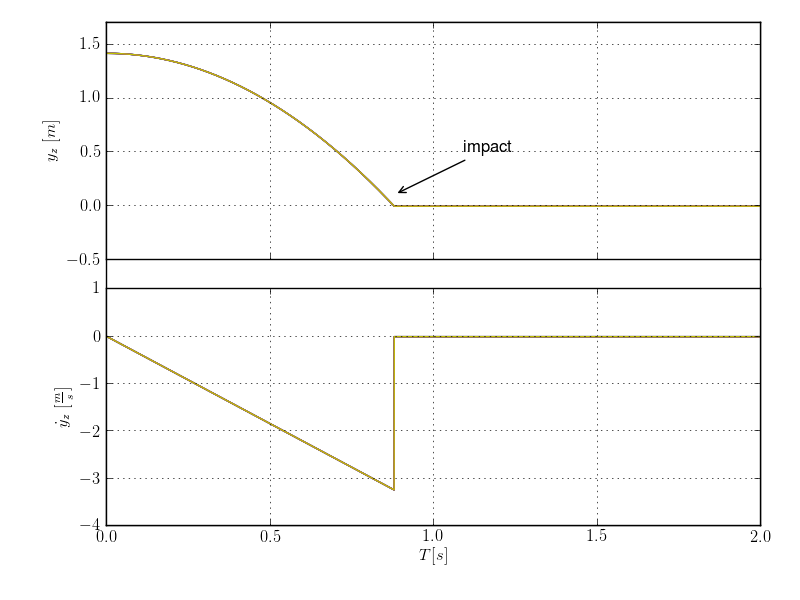
\includegraphics[width=0.8\textwidth]{yNyNdot2}
  \caption{$y_{N}$ - gap function (distance between contact point and the constraint function) for each wheel}
\end{figure}

\noindent \textbf{\textit{\Large{Comments}}}\\[1mm]
\noindent In the figure 12 one can observe one impulsion (force) peak corresponding to the impact when the rover falls onto the ground. In the figure 13 the gap function and relative velocity are diplayed.



\newpage
\section{Test 3}
\label{Sec:test_3}

In the third test setting rover's parcour is divided into six time intervals with different values of torques applied to the wheels:

\begin{enumerate} 
  \item $0s < t_s < 20s$, $\tau = 0Nm$           
  \item $20s < t_s < 40s$, $\tau = 0.0007Nm$        
  \item $40s < t_s < 80s$, $\tau = 0Nm$         
  \item $80s < t_s < 105s$, $\tau = -0.0007Nm$
  \item $105s < t_s < 150s$, $\tau = 0Nm$         
  \item $150s < t_s < 200s$, $\tau = -0.0005Nm$ 
\end{enumerate}

\noindent Other external forces acting on the rover are the gravity and ground reactions. Initial position of the center of mass of the robot
has been set to (x, y, z) = (5, 8, 0.57) [m]. In the $5^{th}$ phase rover effectively stops its motion until negative torques are applied.
Friction coefficient has been set to 0.7. Restitution coefficients (tangential and normal) have been set to zero. 

\begin{figure}[H]
  \centering
    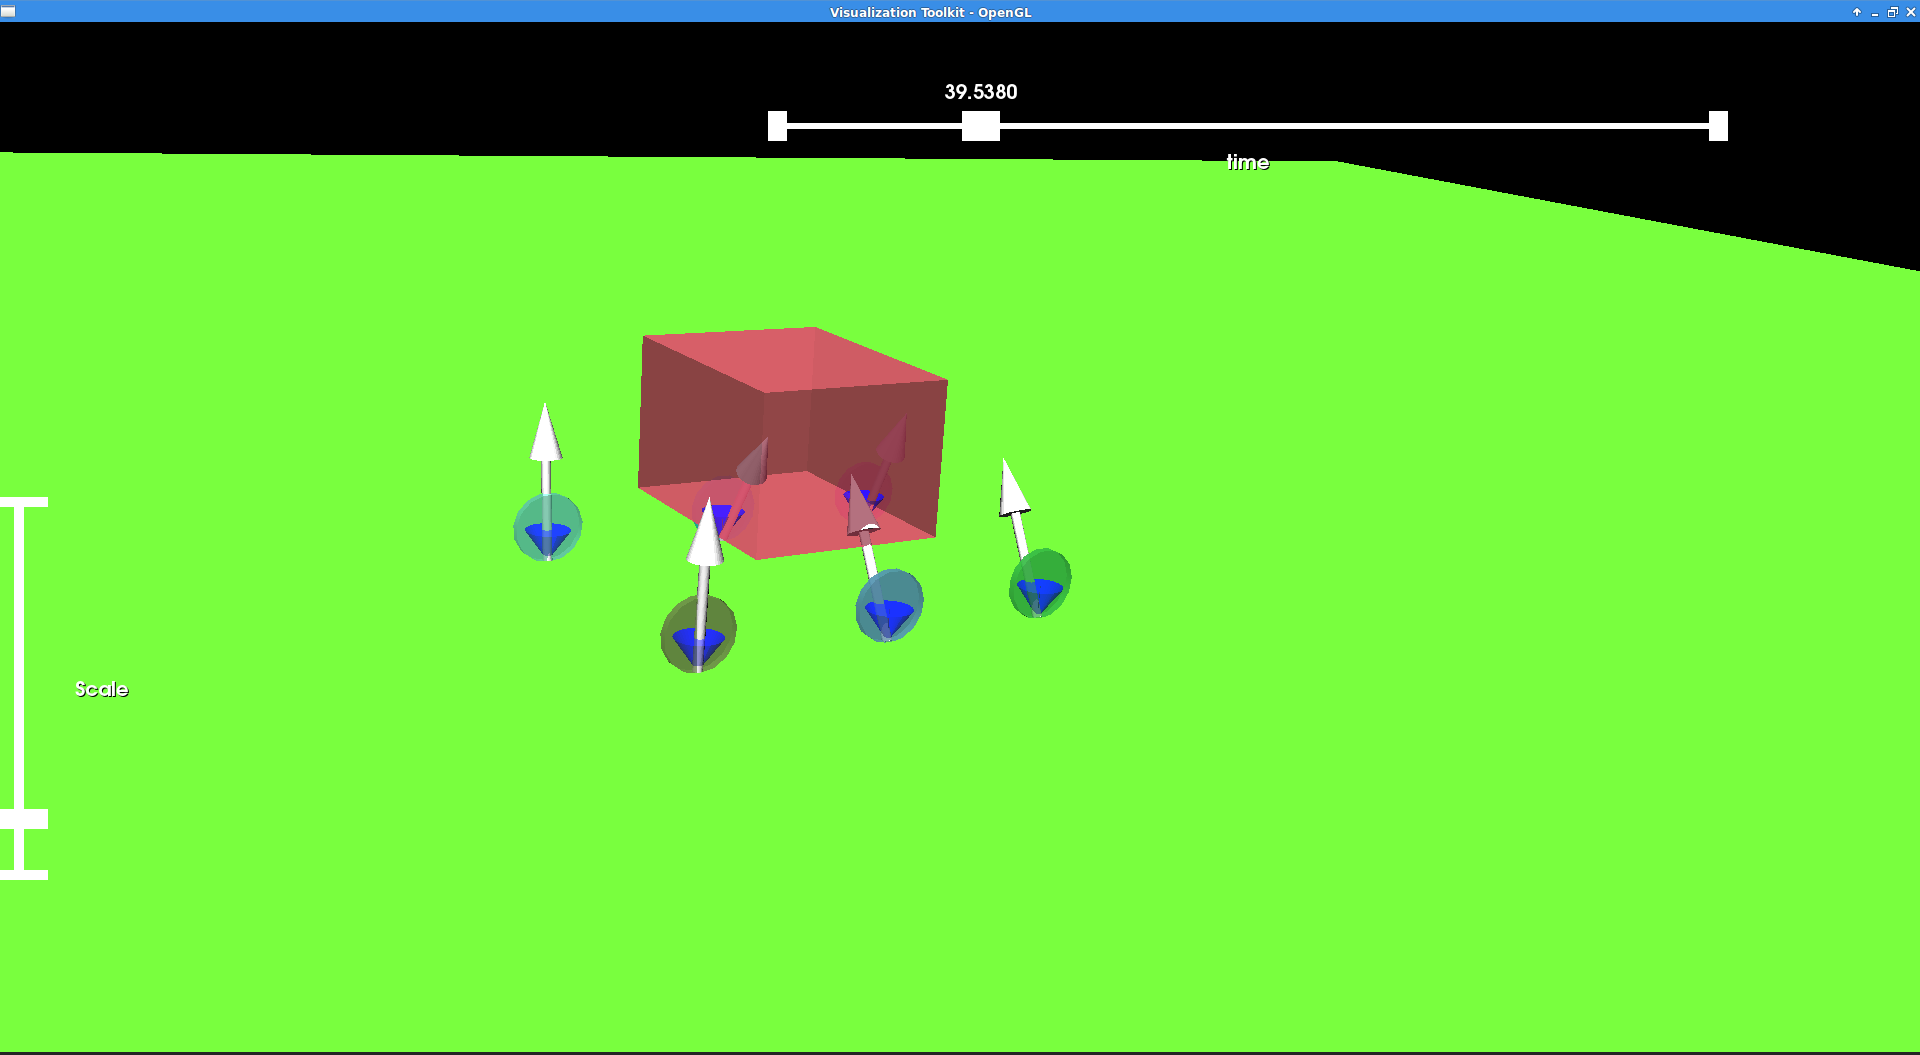
\includegraphics[width=0.8\textwidth]{run_3}
  \caption{Third test scenario (arrows depict contact forces)}
\end{figure}

\noindent In this case, following quantities have been plotted:

\begin{figure}[H]
  \centering
    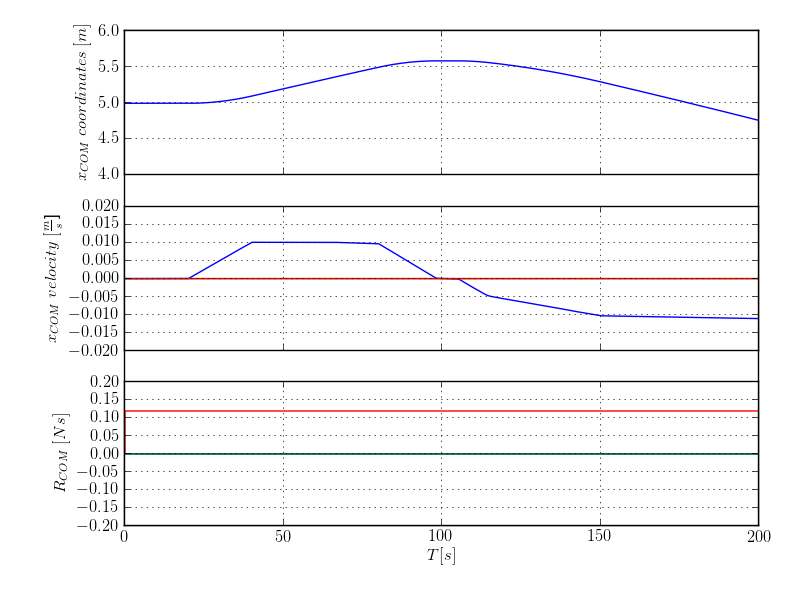
\includegraphics[width=0.8\textwidth]{xvpCOM3}
  \caption{Position, velocity and reaction forces of the center of mass}
\end{figure}

\noindent \textbf{\textit{\Large{Comments}}}\\[1mm]
\noindent Rover's motion has been divided into six phases. Figure 15 depicts those phases in terms of the center of mass velocity. Phases 2 and 3 represent forward motion with 
a constant velocity in the third phase. In the fourth phase rover moves in the opposite direction with a linear velocity to effectively stop in the fifth phase of motion.\\

\noindent Following additional quantities have also been plotted:

\begin{figure}[H]
  \centering
    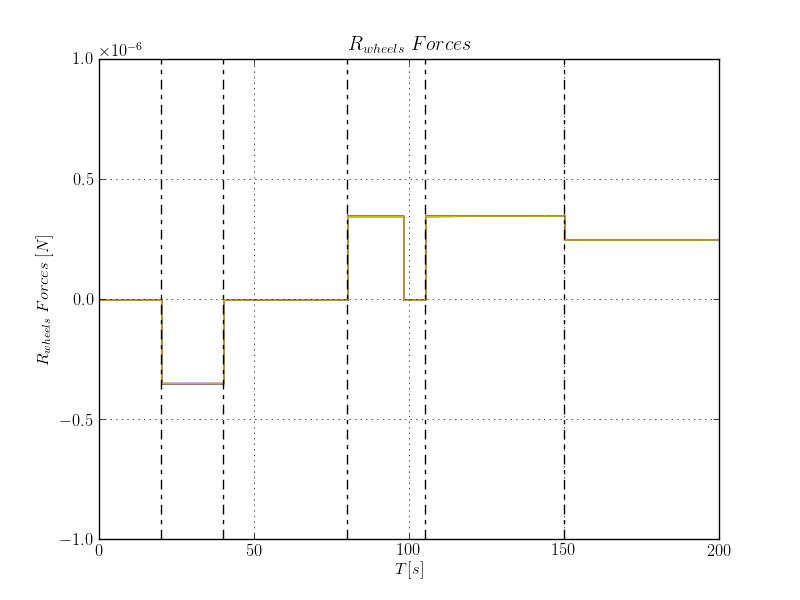
\includegraphics[width=0.8\textwidth]{pWHEELS3}
  \caption{$R_{wheels}$ - reaction forces (impulsions) of wheels in lagrangian coordinates}
\end{figure}

\begin{figure}[H]
  \centering
    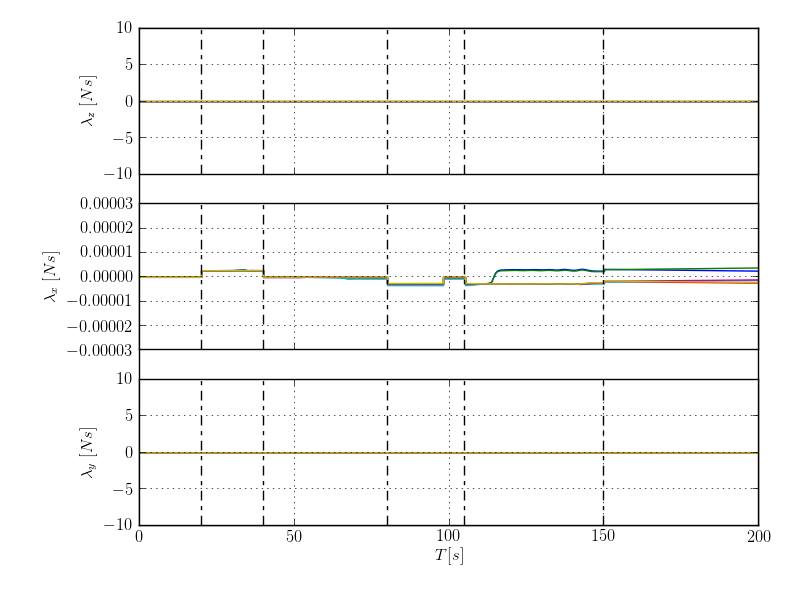
\includegraphics[width=0.8\textwidth]{lambdaNTS3}
  \caption{$\lambda_{N}$, $\lambda_{T_{x}}$, $\lambda_{T_{y}}$ - normal and tangential components of the contact force (impulsion) for each wheel}
\end{figure}

\noindent \textbf{\textit{\Large{Comments}}}\\[1mm]
\noindent In the figure 16 one can see the step pattern of the reaction torques resulting from the fact that the rover is moving along the x axis. Jumps in value represent changes in the friction force along x axis as torques 
are applied to the wheels. In the figure 17 all components of the local contact forces are displayed. Step pattern along x axis can be observed.


\newpage
\section{Test 4}
\label{Sec:test_4}

In the fourth test setting rover stands steadily on the inclined plane.
Inclination angle of the slope has been set to 10$^\circ$. torques applied to the wheels counterbalance torques caused by
the gravity. After initial period higher torques are applied to the wheels which cause the robot to drive upwards.

\begin{figure}[H]
  \centering
    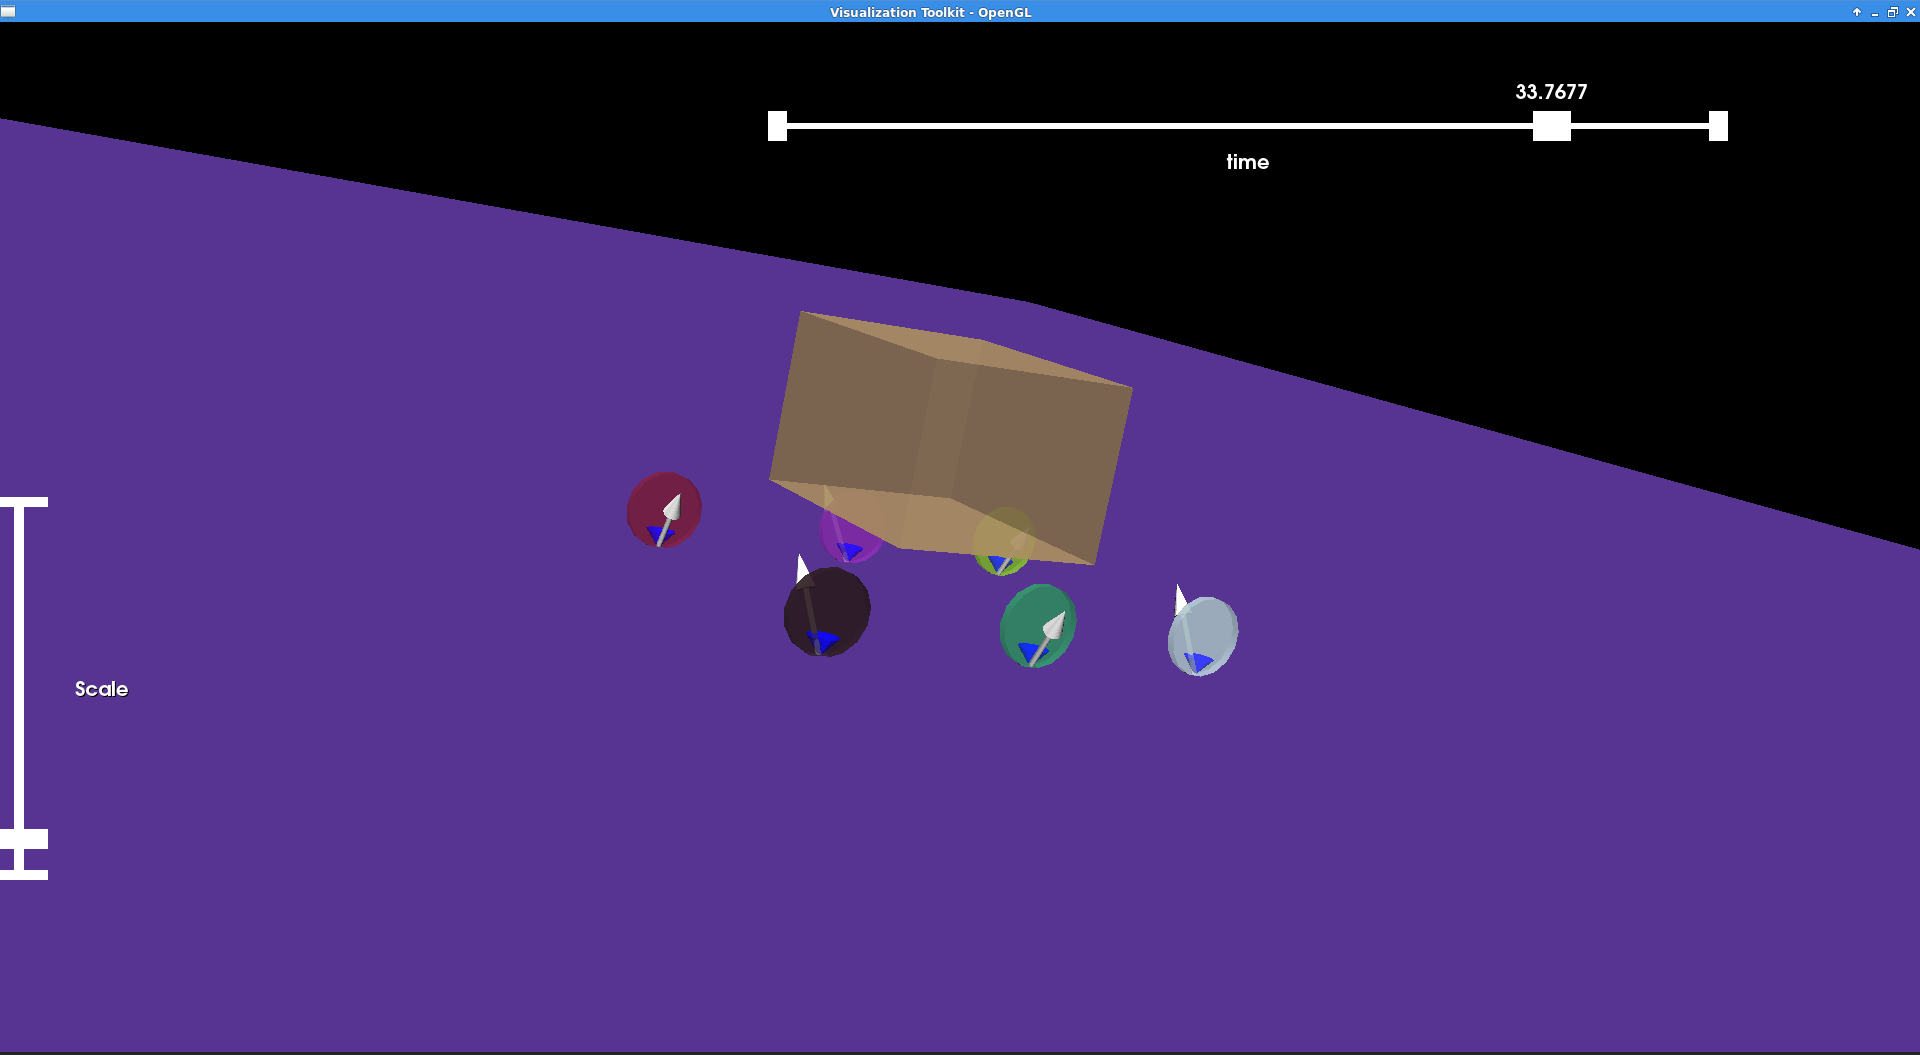
\includegraphics[width=0.8\textwidth]{run_4}
  \caption{Fourth test scenario}
\end{figure}

\noindent Rover's parcour has been devided into two phases:

\begin{enumerate} 
  \item $0s < t_s < 100s$, $\tau = 7495N$           
  \item $100s < t_s < 200s$, $\tau = 10000N$        
\end{enumerate}

\noindent In this case, following quantities have been plotted:

\begin{itemize}
  \item $x_{COM}$ - mass center coordinates
\end{itemize}

\begin{figure}[H]
  \centering
    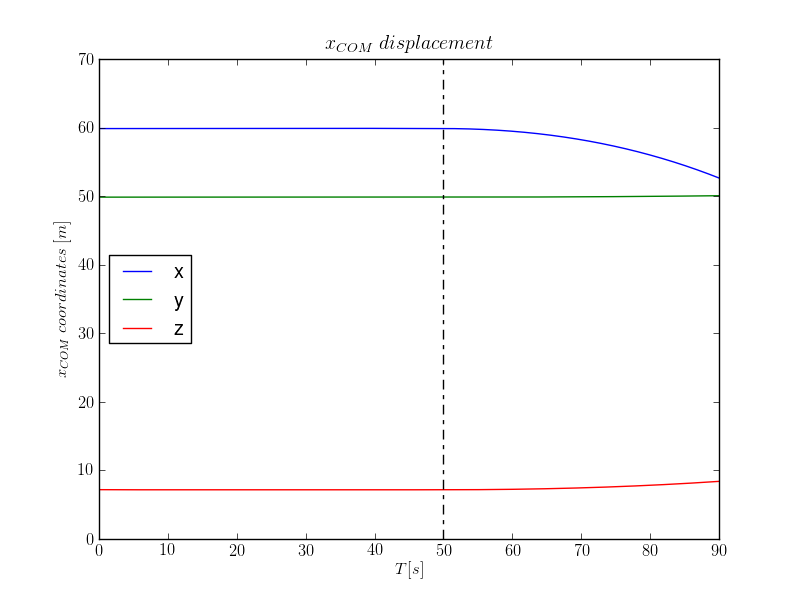
\includegraphics[width=0.8\textwidth]{xCOM4}
  \caption{$x_{COM}$}
\end{figure}

\begin{itemize}
  \item $x_{wheels}$ - wheels angular displacement 
\end{itemize}

\begin{figure}[H]
  \centering
    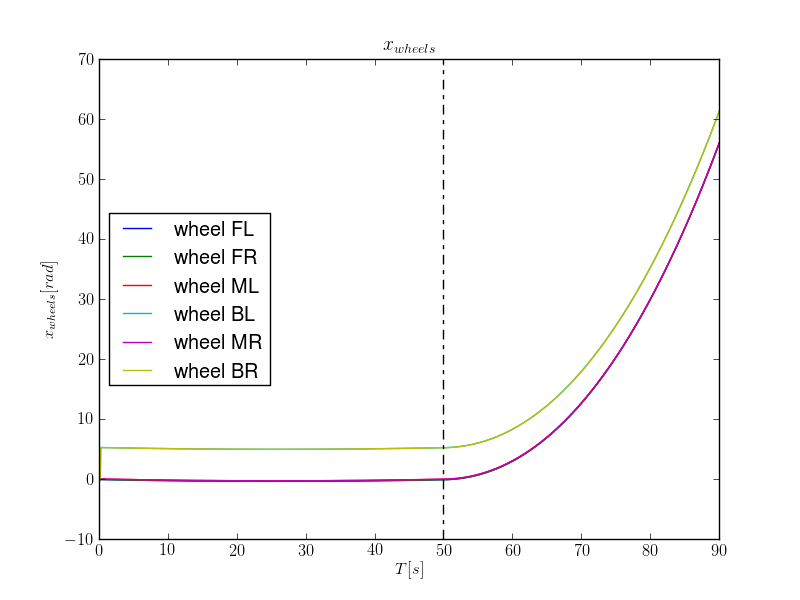
\includegraphics[width=0.8\textwidth]{xWHEELS4}
  \caption{$x_{wheels}$}
\end{figure}

\begin{itemize}
  \item $v_{COM}$ - mass center velocity
\end{itemize}

\begin{figure}[H]
  \centering
    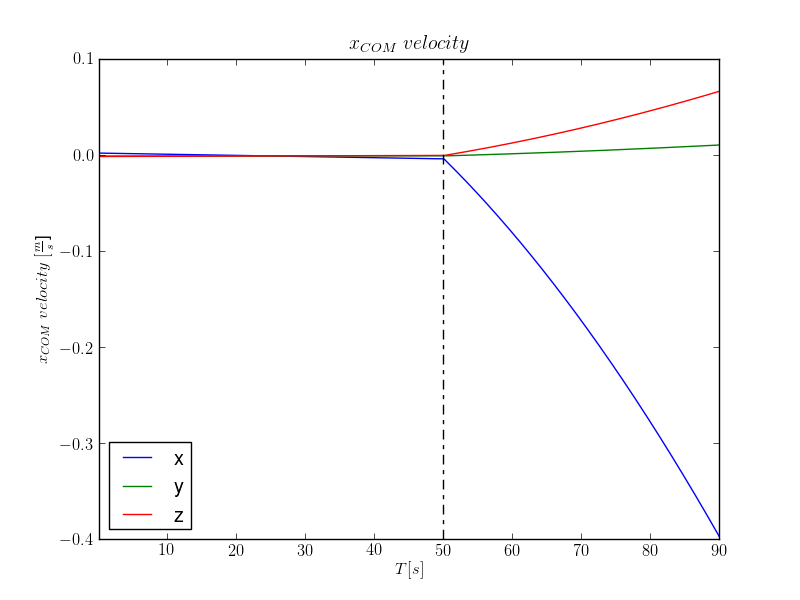
\includegraphics[width=0.8\textwidth]{vCOM4}
  \caption{$v_{COM}$}
\end{figure}

\begin{itemize}
  \item $v_{wheels}$ - wheels angular velocity
\end{itemize}

\begin{figure}[H]
  \centering
    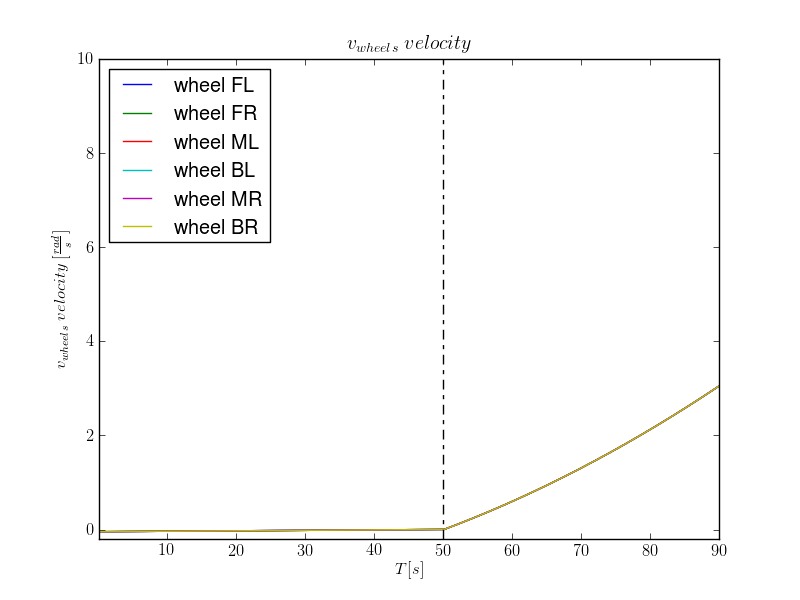
\includegraphics[width=0.8\textwidth]{vWHEELS4}
  \caption{$v_{wheels}$}
\end{figure}

\begin{itemize}
  \item $R_{COM}$ - reaction forces of center of mass in lagrangian coordinates
\end{itemize}

\begin{figure}[H]
  \centering
    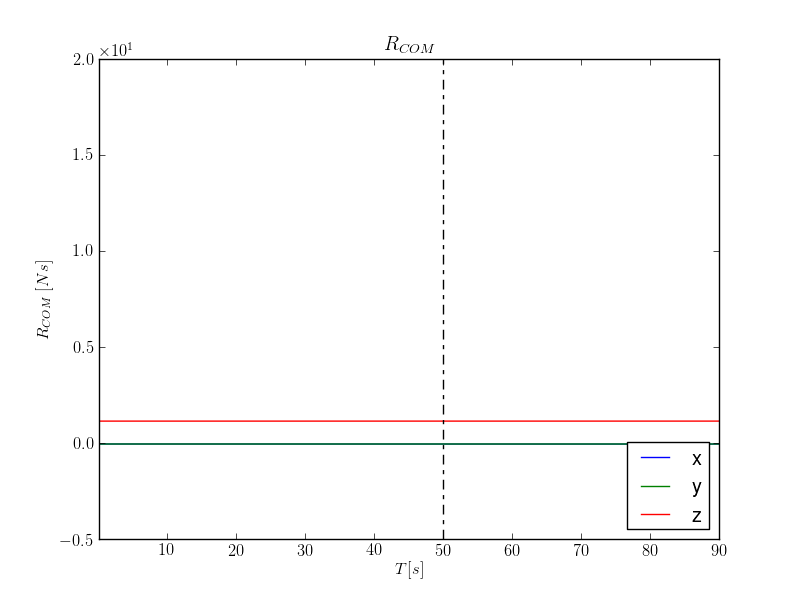
\includegraphics[width=0.8\textwidth]{pCOM4}
  \caption{$R_{COM}$}
\end{figure}

\begin{itemize}
  \item $R_{wheels}$ - reaction forces of wheels in lagrangian coordinates
\end{itemize}

\begin{figure}[H]
  \centering
    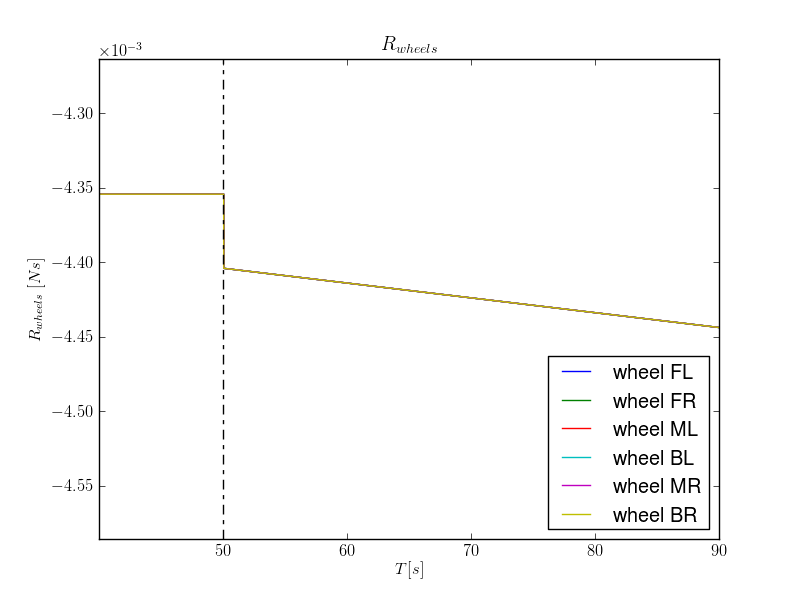
\includegraphics[width=0.8\textwidth]{pWHEELS4}
  \caption{$R_{wheels}$}
\end{figure}

\begin{itemize}
  \item $\lambda_{N}$ - normal component of the contact force (impulsion) for each wheel
\end{itemize}

\begin{figure}[H]
  \centering
    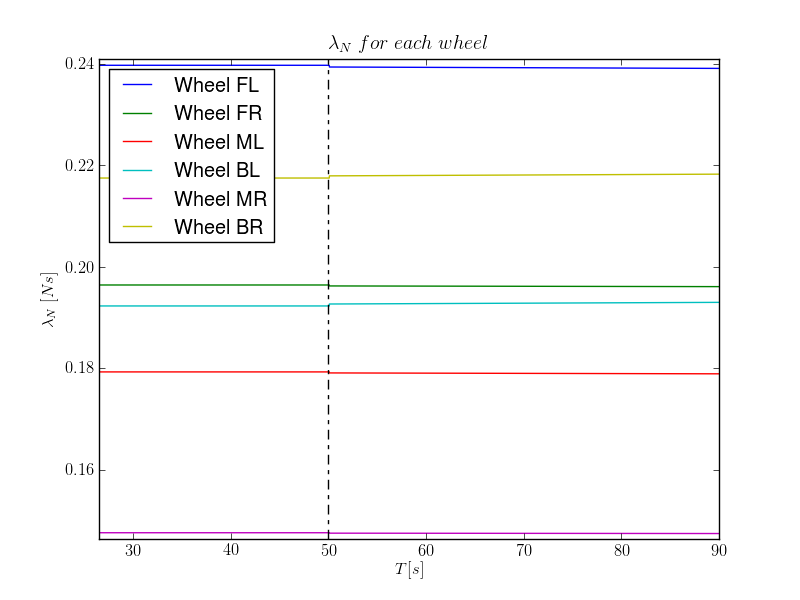
\includegraphics[width=0.8\textwidth]{lambdaN4}
  \caption{$\lambda_N$}
\end{figure}

\begin{itemize}
  \item $\lambda_{T_x}$ - tangential component of the contact force in the x direction for each wheel
\end{itemize}

\begin{figure}[H]
  \centering
    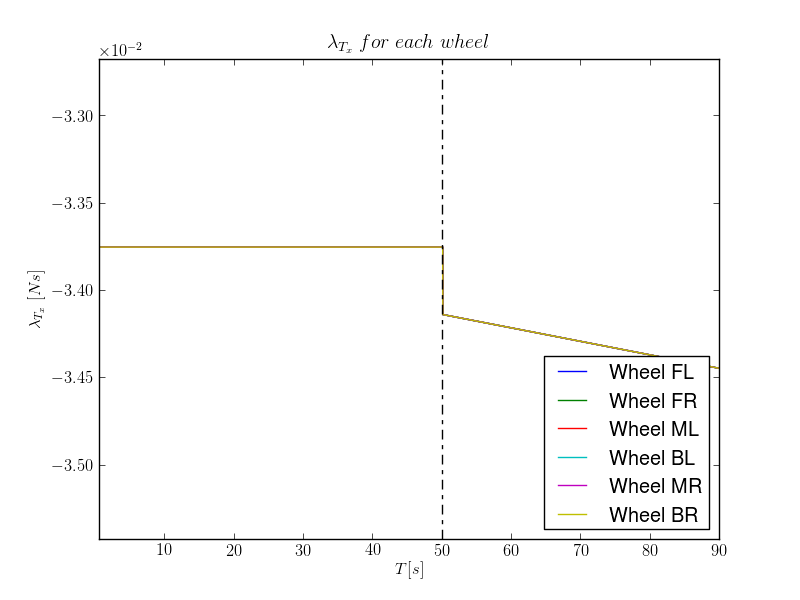
\includegraphics[width=0.8\textwidth]{lambdaTx4}
  \caption{$\lambda_{T_x}$}
\end{figure}

\begin{itemize}
  \item $\lambda_{T_z}$ - tangential component of the contact force in the z direction for each wheel
\end{itemize}

\begin{figure}[H]
  \centering
    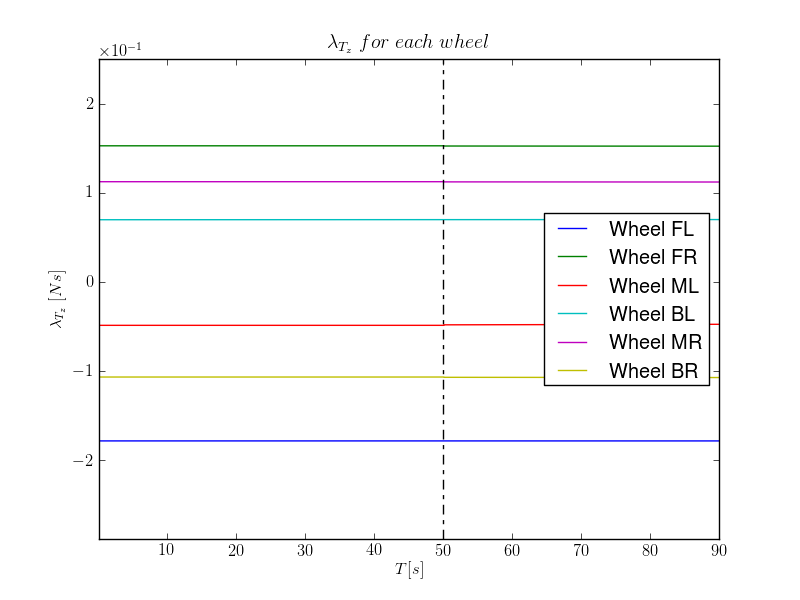
\includegraphics[width=0.8\textwidth]{lambdaTz4}
  \caption{$\lambda_{T_z}$}
\end{figure}

\begin{itemize}
  \item $y_{N}$ - gap function (distance between contact point and the constraint function) for each wheel
\end{itemize}

\begin{figure}[H]
  \centering
    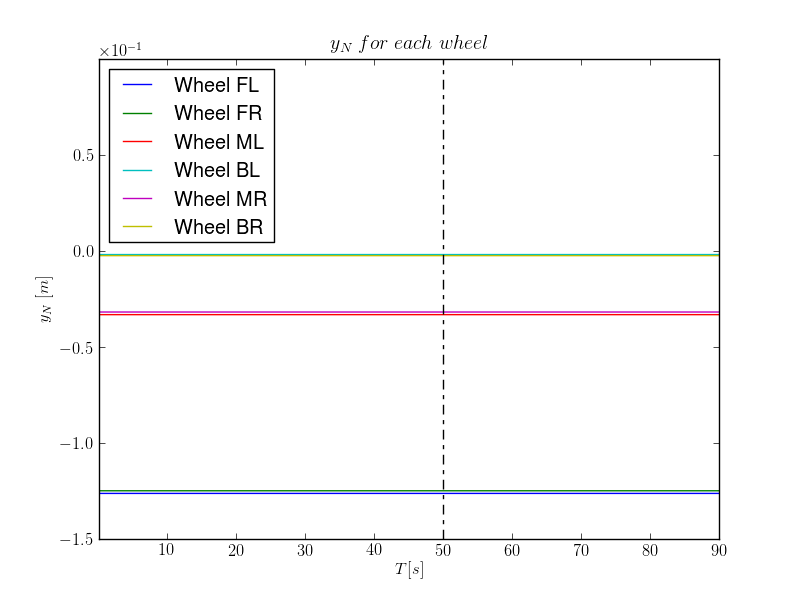
\includegraphics[width=0.8\textwidth]{yN4}
  \caption{$y_N$}
\end{figure}

\begin{itemize}
  \item $\dot{y}_{N}$ - normal component of the local contact velocity for each wheel
\end{itemize}

\begin{figure}[H]
  \centering
    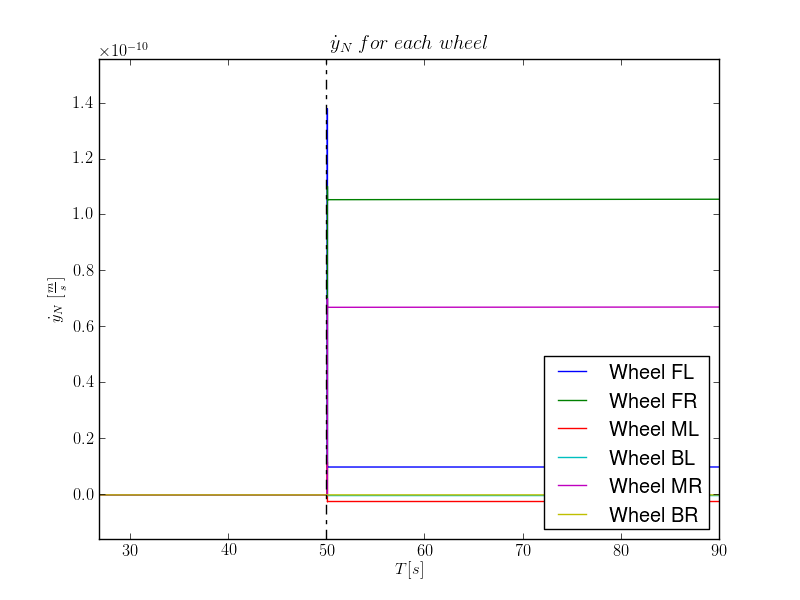
\includegraphics[width=0.8\textwidth]{yNdot4}
  \caption{$\dot{y}_{N}$}
\end{figure}

\begin{itemize}
  \item $\dot{y}_{T_x}$ - tangential component x of the local contact velocity for each wheel
\end{itemize}

\begin{figure}[H]
  \centering
    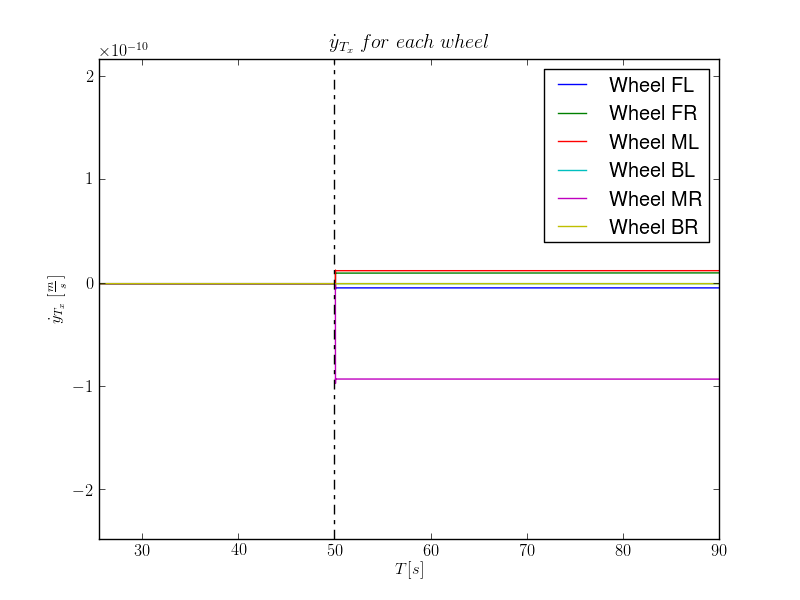
\includegraphics[width=0.8\textwidth]{yTxdots4}
  \caption{$\dot{y}_{T_x}$}
\end{figure}

\begin{itemize}
  \item $\dot{y}_{T_z}$ - tangential component z of the local contact velocity for each wheel
\end{itemize}

\begin{figure}[H]
  \centering
    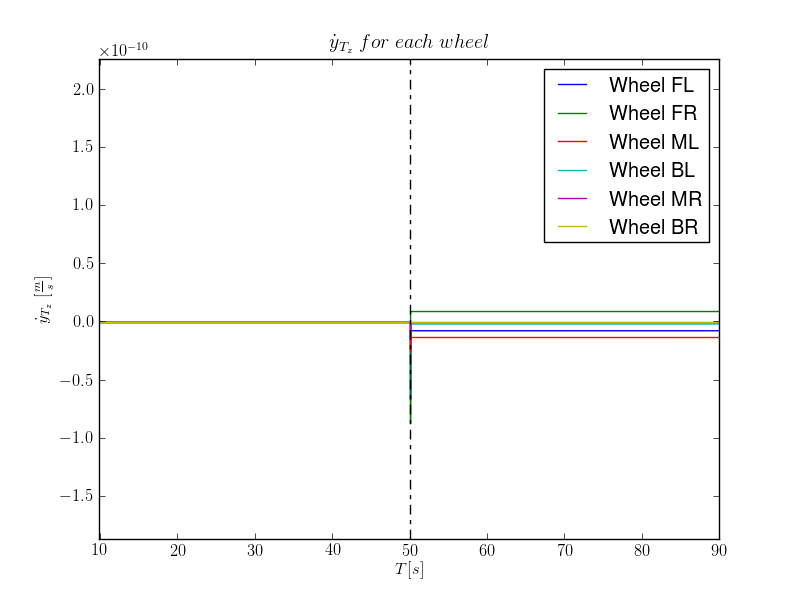
\includegraphics[width=0.8\textwidth]{yTzdots4}
  \caption{$\dot{y}_{T_z}$}
\end{figure}



\newpage
\section{Test 5}
\label{Sec:test_5}

In the fifth test setting rover is dropped onto the inclined plane.
Inclination angle of the slope has been set to 10$^\circ$. After 5$^{th}$ second of motion a simple PD controller
is set on in order to stop the rover on the slope. Rover stops effectively at $t = 119.965s$. At $t = 200s$ constant torques has been applied to all the wheels.
Values of applied torques equaled $\tau = 9500Nm$. Hence, Since $t = 200s$ rover drives upwards. 

\begin{figure}[H]
  \centering
    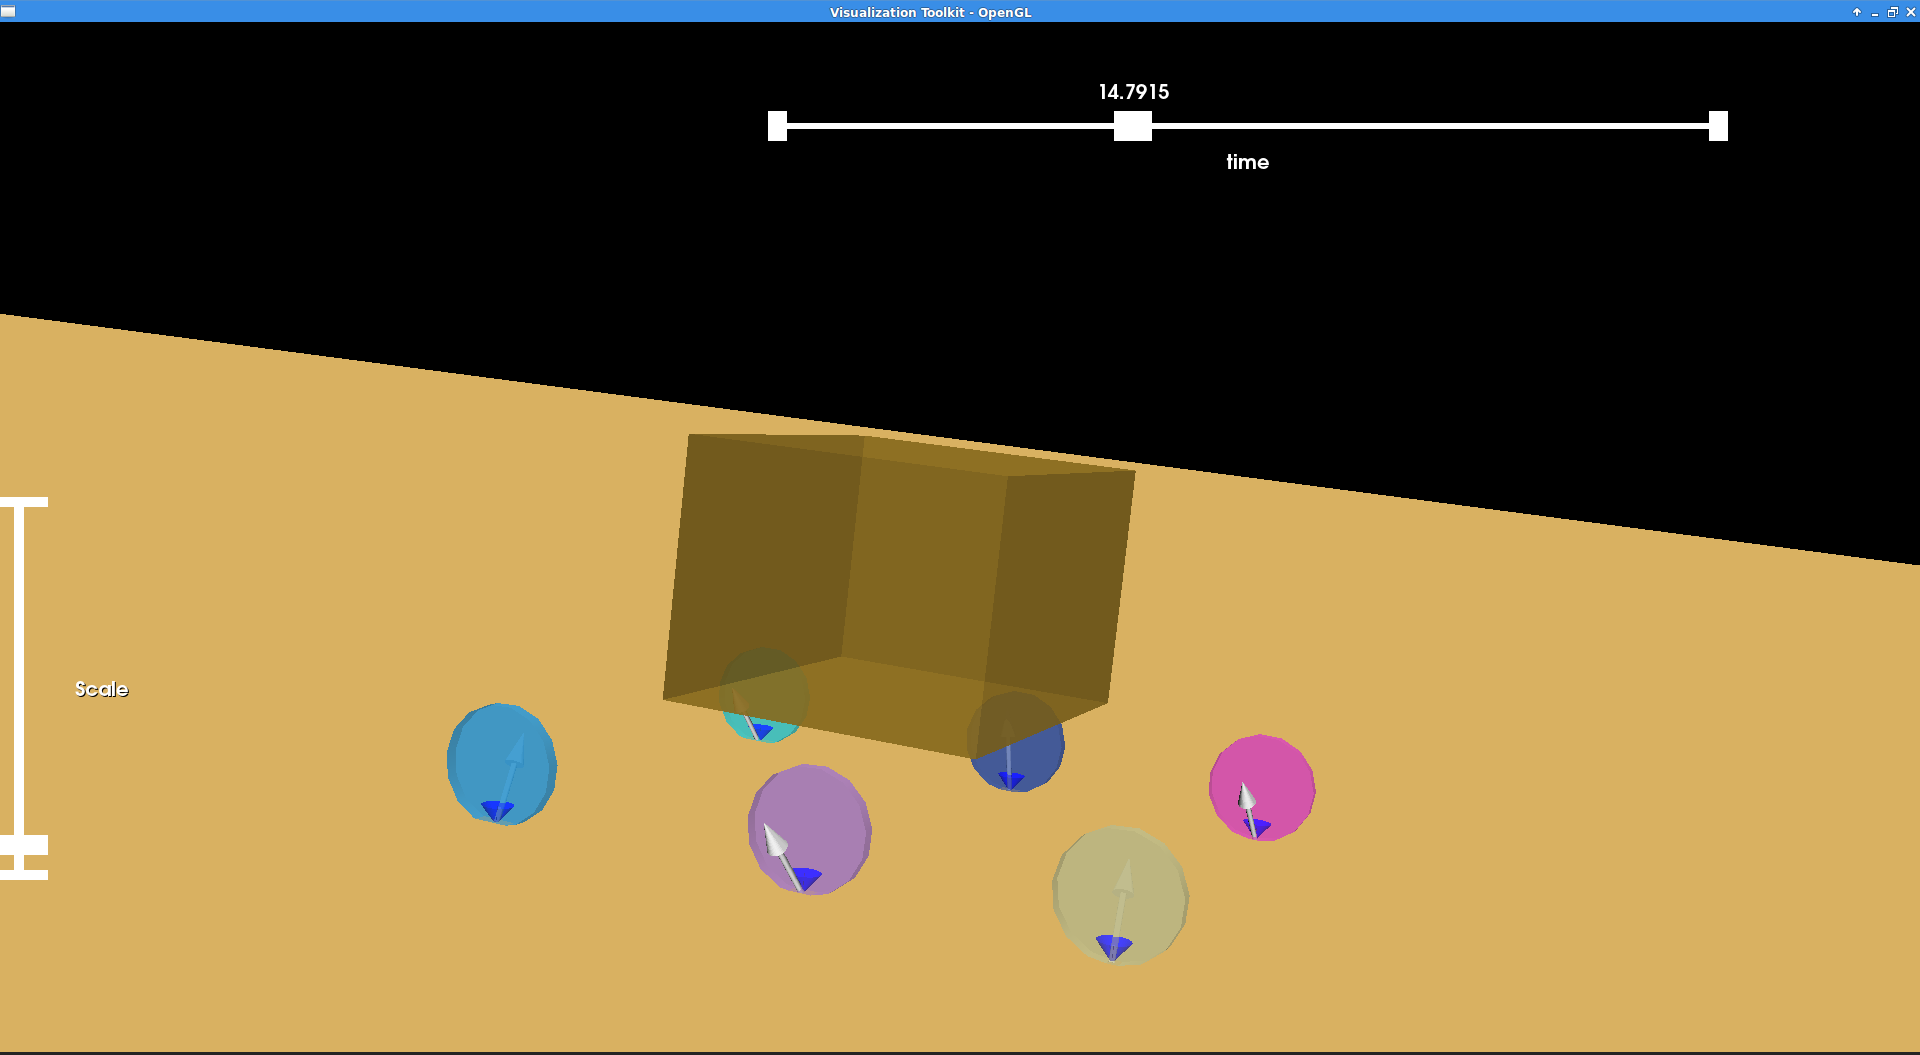
\includegraphics[width=0.8\textwidth]{run_5}
  \caption{Fifth test scenario}
\end{figure}

\noindent  In this setting we are mostly interested in two phases:

\begin{enumerate} 
  \item $119.965s < t_s < 200s$
  \item $200s < t_s < 300s$
\end{enumerate}

\noindent In this case, following quantities have been plotted:

\begin{itemize}
  \item $x_{COM}$ - mass center coordinates
\end{itemize}

\begin{figure}[H]
  \centering
    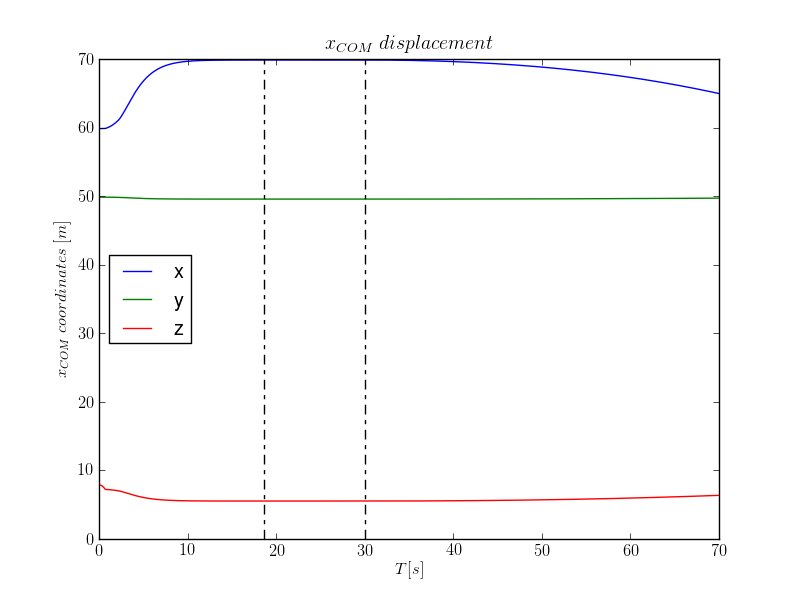
\includegraphics[width=0.8\textwidth]{xCOM5}
  \caption{$x_{COM}$}
\end{figure}

\begin{itemize}
  \item $x_{wheels}$ - wheels angular displacement 
\end{itemize}

\begin{figure}[H]
  \centering
    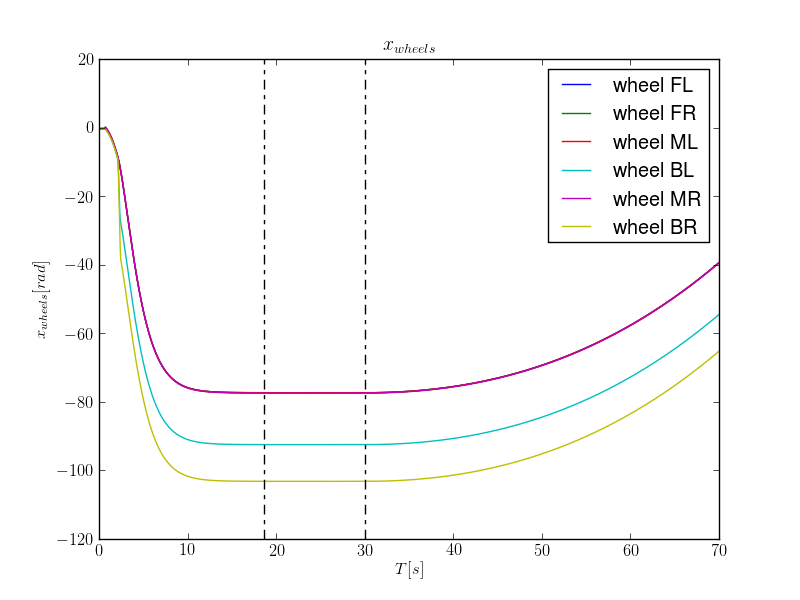
\includegraphics[width=0.8\textwidth]{xWHEELS5}
  \caption{$x_{wheels}$}
\end{figure}

\begin{itemize}
  \item $v_{COM}$ - mass center velocity
\end{itemize}

\begin{figure}[H]
  \centering
    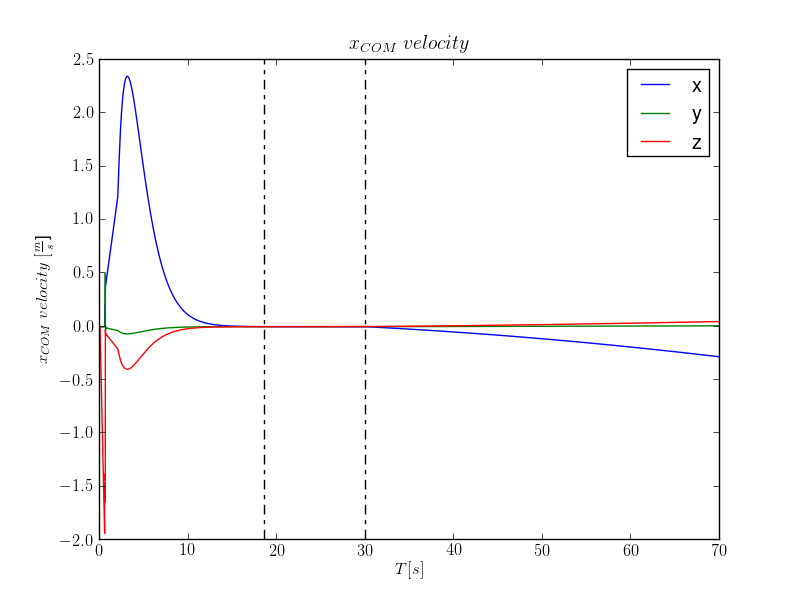
\includegraphics[width=0.8\textwidth]{vCOM5}
  \caption{$v_{COM}$}
\end{figure}

\begin{itemize}
  \item $v_{wheels}$ - wheels angular velocity
\end{itemize}

\begin{figure}[H]
  \centering
    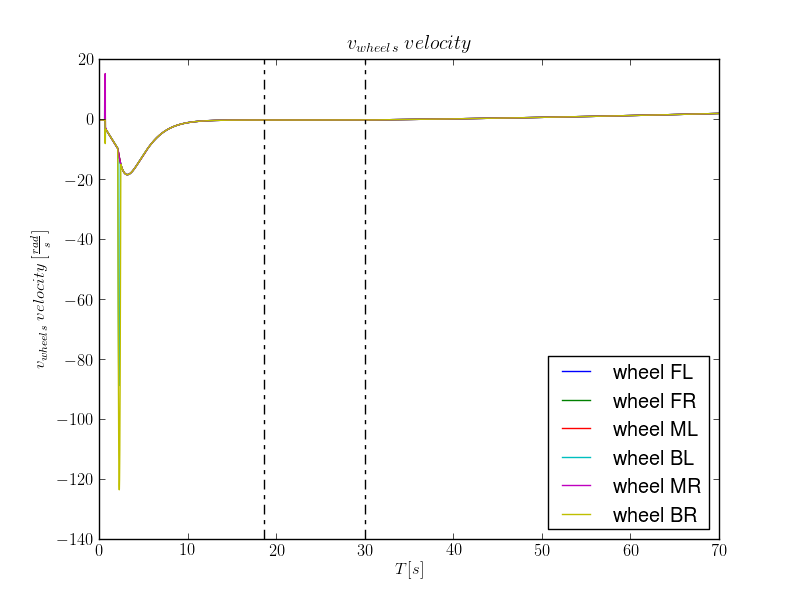
\includegraphics[width=0.8\textwidth]{vWHEELS5}
  \caption{$v_{wheels}$}
\end{figure}

\begin{itemize}
  \item $R_{COM}$ - reaction forces of center of mass in lagrangian coordinates
\end{itemize}

\begin{figure}[H]
  \centering
    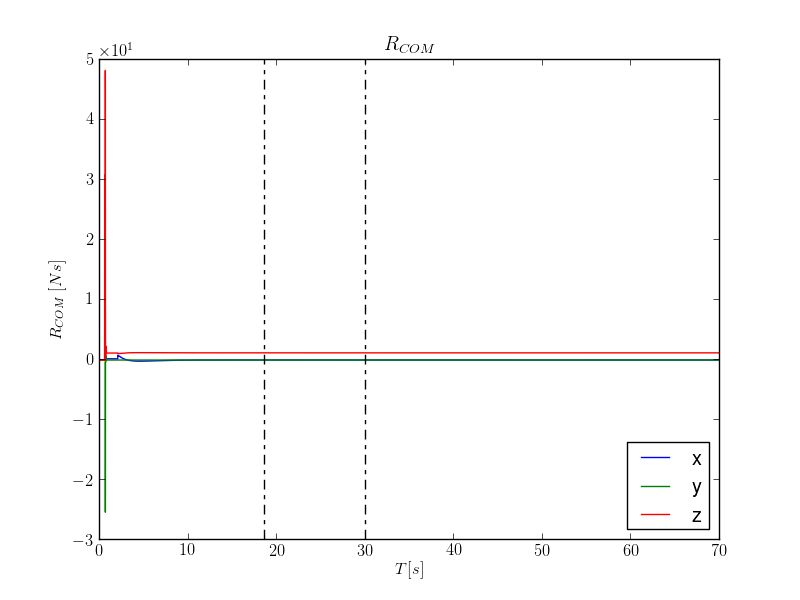
\includegraphics[width=0.8\textwidth]{pCOM5}
  \caption{$R_{COM}$}
\end{figure}

\begin{figure}[H]
  \centering
    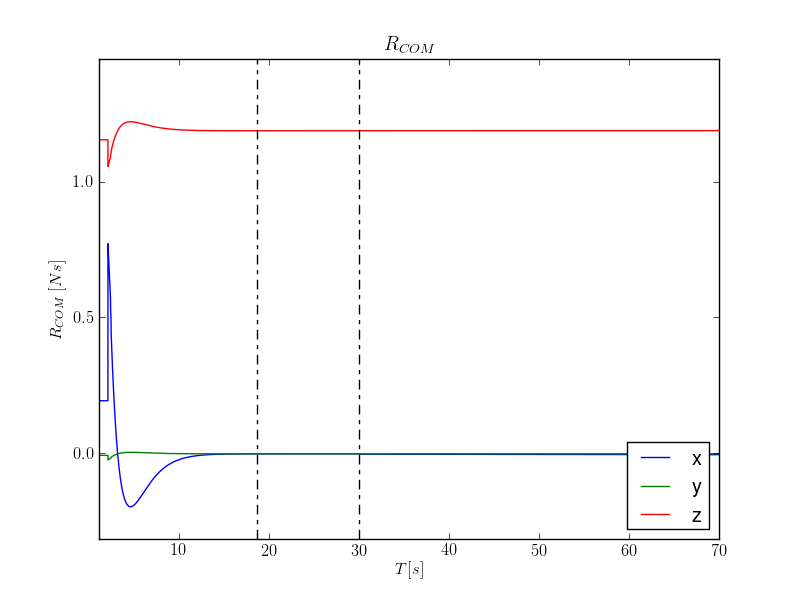
\includegraphics[width=0.8\textwidth]{pCOM5postimpact}
  \caption{$R_{COM}$ without impact part}
\end{figure}

\begin{itemize}
  \item $R_{wheels}$ - reaction forces of wheels in lagrangian coordinates
\end{itemize}

\begin{figure}[H]
  \centering
    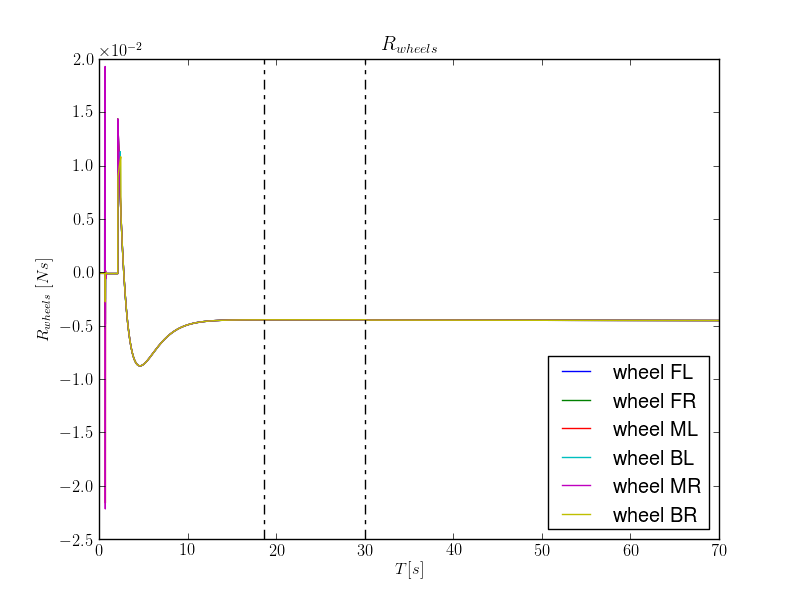
\includegraphics[width=0.8\textwidth]{pWHEELS5}
  \caption{$R_{wheels}$}
\end{figure}

\begin{itemize}
  \item $\lambda_{N}$ - normal component of the contact force (impulsion) for each wheel
\end{itemize}

\begin{figure}[H]
  \centering
    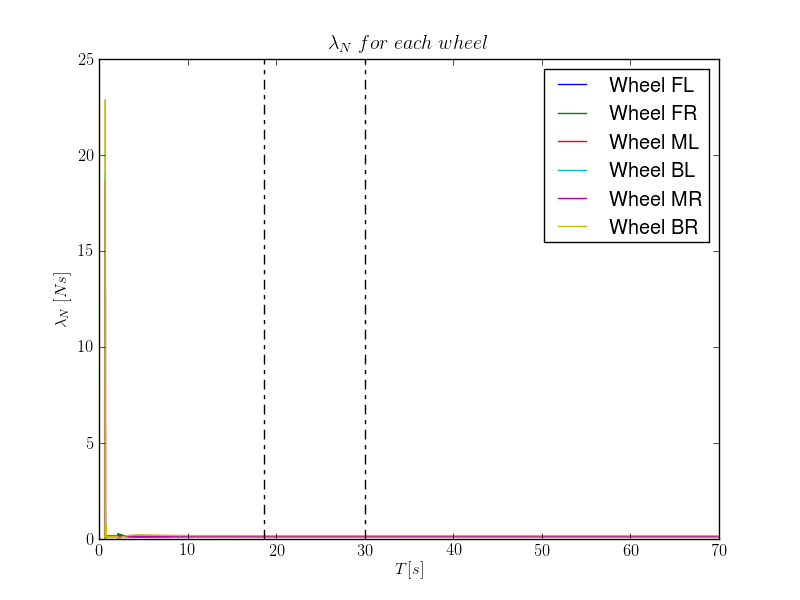
\includegraphics[width=0.8\textwidth]{lambdaN5}
  \caption{$\lambda_N$}
\end{figure}

\begin{figure}[H]
  \centering
    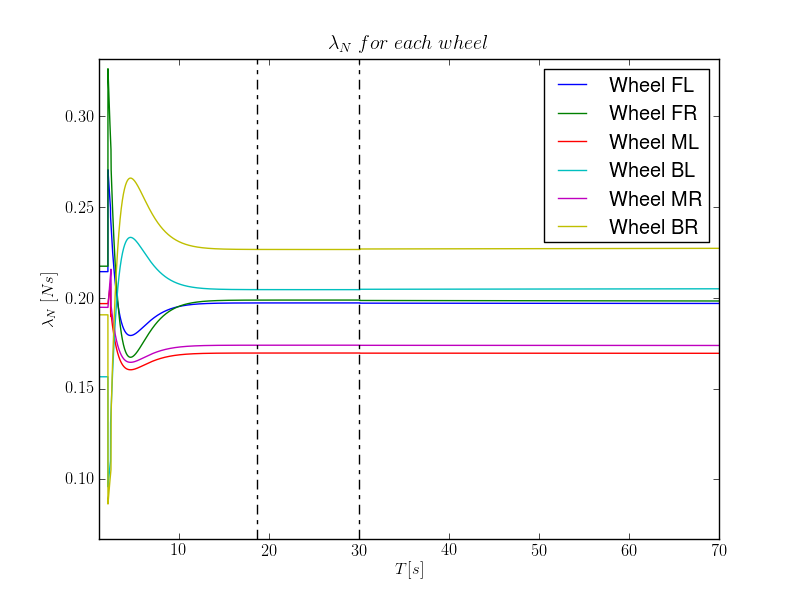
\includegraphics[width=0.8\textwidth]{lambdaN5zoom}
  \caption{$\lambda_N$ without impact phase}
\end{figure}

\begin{itemize}
  \item $\lambda_{T_x}$ - tangential component of the contact force in the x direction for each wheel
\end{itemize}

\begin{figure}[H]
  \centering
    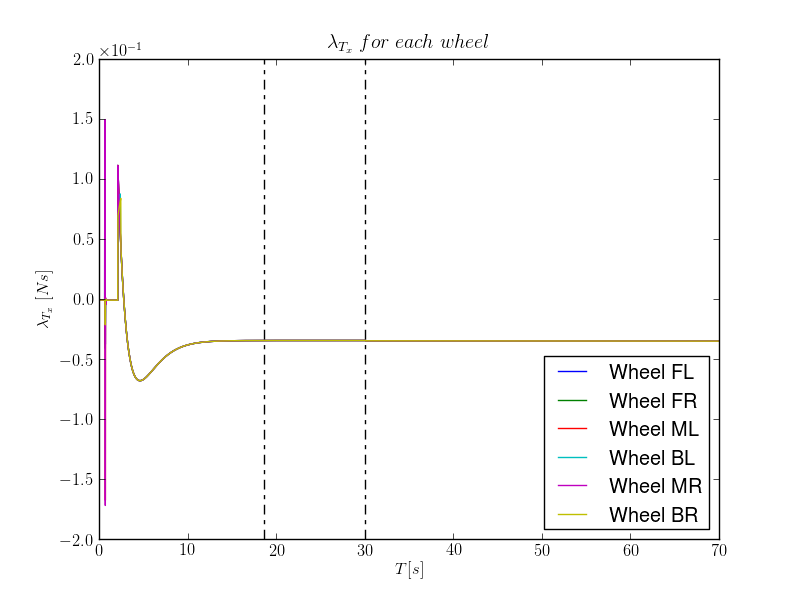
\includegraphics[width=0.8\textwidth]{lambdaTx5}
  \caption{$\lambda_{T_x}$}
\end{figure}

\begin{itemize}
  \item $\lambda_{T_z}$ - tangential component of the contact force in the z direction for each wheel
\end{itemize}

\begin{figure}[H]
  \centering
    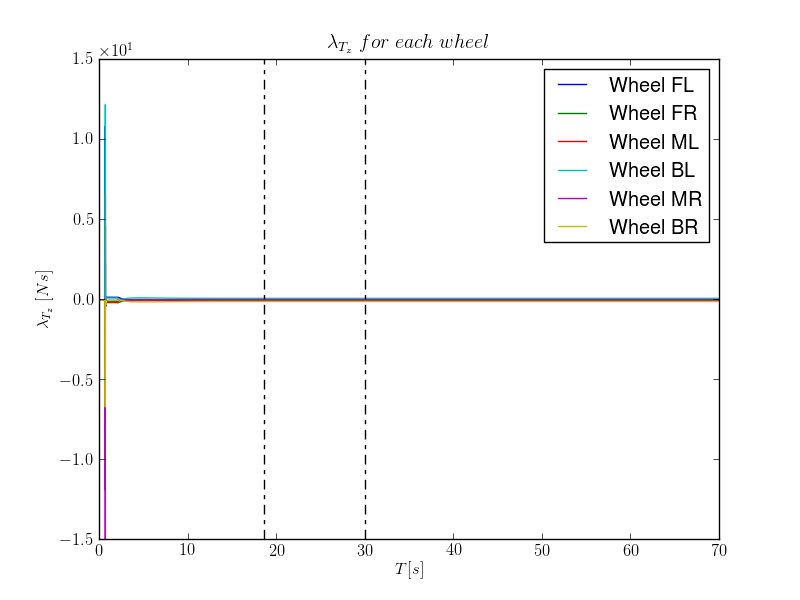
\includegraphics[width=0.8\textwidth]{lambdaTz5}
  \caption{$\lambda_{T_z}$}
\end{figure}

\begin{figure}[H]
  \centering
    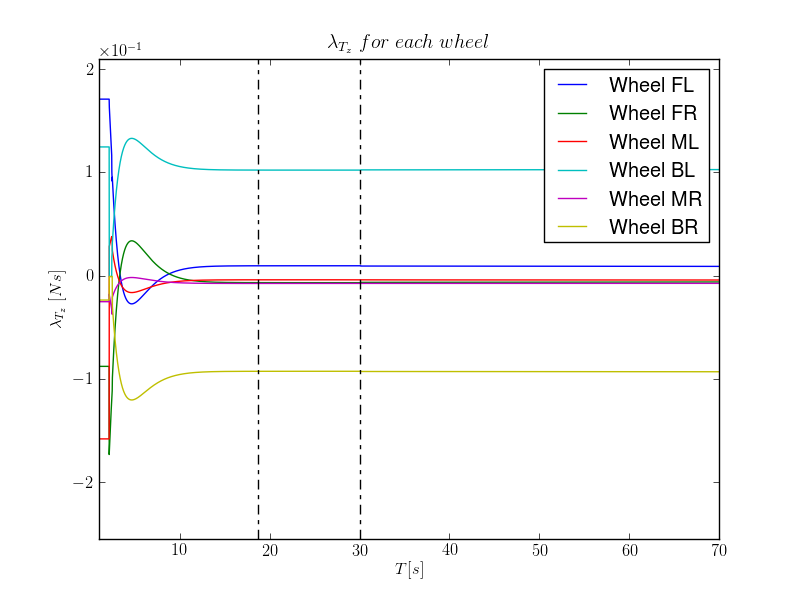
\includegraphics[width=0.8\textwidth]{lambdaTz5zoom}
  \caption{$\lambda_{T_z}$ without impact phase}
\end{figure}

\begin{itemize}
  \item $y_{N}$ - gap function (distance between contact point and the constraint function) for each wheel
\end{itemize}

\begin{figure}[H]
  \centering
    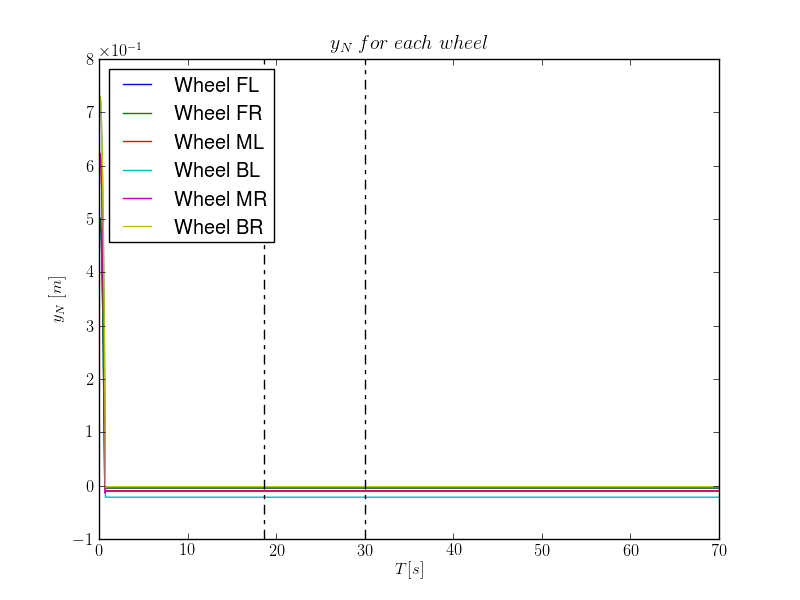
\includegraphics[width=0.8\textwidth]{yN5}
  \caption{$y_N$}
\end{figure}

\begin{figure}[H]
  \centering
    \includegraphics[width=0.8\textwidth]{yN5zoom}
  \caption{$y_N$ after impact phase}
\end{figure}

\begin{itemize}
  \item $\dot{y}_{N}$ - normal component of the local contact velocity for each wheel
\end{itemize}

\begin{figure}[H]
  \centering
    \includegraphics[width=0.8\textwidth]{yNdot5}
  \caption{$\dot{y}_{N}$}
\end{figure}

\begin{itemize}
  \item $\dot{y}_{T_x}$ - tangential component x of the local contact velocity for each wheel
\end{itemize}

\begin{figure}[H]
  \centering
    \includegraphics[width=0.8\textwidth]{yTxdots5}
  \caption{$\dot{y}_{T_x}$}
\end{figure}

\begin{itemize}
  \item $\dot{y}_{T_z}$ - tangential component z of the local contact velocity for each wheel
\end{itemize}

\begin{figure}[H]
  \centering
    \includegraphics[width=0.8\textwidth]{yTzdots5}
  \caption{$\dot{y}_{T_z}$}
\end{figure}



\newpage
\section{Test 6}
\label{Sec:test_6}

In the sixth test setting rover is dropped onto the horizontal plane from the height of $2$ $m$. After $10$ $s$ linearly varying torques are applied to all wheels. 
A spherical obstacle has been set in front of the rover. The obstacle is in the form of a sphere which protudes outside the plane.
Center of the sphere has been set so that the protrusion is equal to $20$ $cm$. Coefficient of friction has been set to 0.3 whereas the coefficient of restitution to 0.

\begin{figure}[H]
  \centering
    \includegraphics[width=0.8\textwidth]{run_6}
  \caption{Sixth test scenario}
\end{figure}

\noindent In this case, the following essential quantities have been plotted:

\begin{figure}[H]
  \centering
    \includegraphics[width=0.8\textwidth]{xvpCOM6}
  \caption{position, velocity and reaction forces of the mass center of the rover}
\end{figure}

\noindent \textbf{\textit{\Large{Comments}}}\\[1mm]
\noindent In this setting attention can be drawn to the spherical obstacle crossing. In the figure 27 in the first sub-plot on can see $z$ coordinate evolution of the mass center of the robot. 
It is clearly seen how around 11$^{th}$ minute rover mounts the sphere. In the sub-plot below one can see the evolution of velocities of the mass center where several small jumps occur in the 
$y$ and $z$ dimension as a result of impacts. Velocity in the $x$ direction is clearly larger as the rover moves along the $x$ axis. Impacts are more clearly seen in the third sub-plot with each peak 
corresponding to an impact.\\
 
\noindent Following additional quantities have also been plotted:

\begin{figure}[H]
  \centering
    \includegraphics[width=0.8\textwidth]{lambdaNTS6}
  \caption{$\lambda_{N}$, $\lambda_{T_x}$, $\lambda_{T_y}$ - normal component of the contact force (impulsion) for each wheel (interaction with the plane)}
\end{figure}

\begin{figure}[H]
  \centering
    \includegraphics[width=0.8\textwidth]{lambdaNTS6sphere}
  \caption{$\lambda_{N}$, $\lambda_{T_x}$, $\lambda_{T_y}$ - normal component of the contact force (impulsion) for each wheel (interaction with the sphere)}
\end{figure}

\noindent \textbf{\textit{\Large{Comments}}}\\[1mm]
\noindent In the figure 28 and 29 local contact forces have been plotted seen from the interaction with plane and sphere respectively. One can observe several peaks corresponding to the
phase of the simulation when the obstacle is being crossed.\\


\newpage
\section{Test 7}
\label{Sec:test_7}

In the seveth test setting rover is dropped onto the horizontal plane.
An obstacle in the form of a horizontal step of height $0.1$ $m$ has been set in front of the rover.
At certain point rover starts moving towards the step and crosses it mounting on the higher plane.

\begin{figure}[H]
  \centering
    \includegraphics[width=0.8\textwidth]{run_7}
  \caption{Seventh test scenario}
\end{figure}

\noindent In this case, following quantities have been plotted:

\begin{itemize}
  \item $x_{COM}$ - mass center coordinates
\end{itemize}

\begin{figure}[H]
  \centering
    \includegraphics[width=0.8\textwidth]{xCOM7}
  \caption{$x_{COM}$}
\end{figure}

\begin{itemize}
  \item $x_{wheels}$ - wheels angular displacement 
\end{itemize}

\begin{figure}[H]
  \centering
    \includegraphics[width=0.8\textwidth]{xWHEELS7}
  \caption{$x_{wheels}$}
\end{figure}

\begin{itemize}
  \item $v_{COM}$ - mass center velocity
\end{itemize}

\begin{figure}[H]
  \centering
    \includegraphics[width=0.8\textwidth]{vCOM7}
  \caption{$v_{COM}$}
\end{figure}

\begin{itemize}
  \item $v_{wheels}$ - wheels angular velocity
\end{itemize}

\begin{figure}[H]
  \centering
    \includegraphics[width=0.8\textwidth]{vWHEELS7}
  \caption{$v_{wheels}$}
\end{figure}

\begin{itemize}
  \item $R_{COM}$ - reaction forces of center of mass in lagrangian coordinates
\end{itemize}

\begin{figure}[H]
  \centering
    \includegraphics[width=0.8\textwidth]{pCOM7}
  \caption{$R_{COM}$}
\end{figure}

\begin{itemize}
  \item $R_{wheels}$ - reaction forces of wheels in lagrangian coordinates
\end{itemize}

\begin{figure}[H]
  \centering
    \includegraphics[width=0.8\textwidth]{pWHEELS7}
  \caption{$R_{wheels}$}
\end{figure}


\end{document}
 
